\section{特異値分解}

\begin{frame}[t,fragile]{一般の非正方行列の場合}
  \begin{itemize}
    %\setlength{\itemsep}{1em}
  \item 特異値分解(SVD: Singular Value Decomposition)
  \item 任意の$m \times n$実行列$A$は
    \[
    A = U \Lambda V^T
    \]
    の形に(一意に)分解できる ($k=\min(m,n)$)
  \item $U$: $(m \times k)$行列(列ベクトルは互いに正規直交) \\
    $V$: $(n \times k)$行列(列ベクトルは互いに正規直交) \\
    $\Lambda = \text{diag}(\lambda_1,\lambda_2,\cdots,\lambda_k)$ \ \ ($\lambda_1\ge\lambda_2\ge\cdots\ge\lambda_k\ge 0$) 特異値
  \item ベクトル表示 (行列をランク1の行列で分解)
    \[
    A = \sum_{i=1}^k \lambda_i u_i v_i^{T}
    \]
  \end{itemize}
\end{frame}

\begin{frame}[t,fragile]{特異値分解の例}
  \[
  \begin{split}
    \begin{pmatrix}
      1 & 2 & 3 \\
      6 & 4 & 5 \\
      8 & 9 & 7 \\
      10 & 11 & 12
    \end{pmatrix} =&
    \begin{pmatrix}
      -0.14 & -0.62 & -0.05 \\
      -0.34 & \ \ \,0.37 & \ \ \,0.81 \\
      -0.55 & \ \ \,0.54 & -0.58 \\
      -0.75 & -0.44 & \ \ \,0.06      
    \end{pmatrix} \\
    &\times
    \begin{pmatrix}
      25.35 & 0 & 0 \\
      0 & 2.15 & 0 \\
      0 & 0 & 1.71
    \end{pmatrix}
    \begin{pmatrix}
      -0.56 & -0.59 & -0.59 \\
      \ \ \,0.68 & \ \ \,0.09 & -0.73 \\
      \ \ \,0.48 & -0.81 & \ \ \,0.35
    \end{pmatrix}
  \end{split}
  \]
\end{frame}

\begin{frame}[t,fragile]{完全特異値分解 (full SVD)}
  \[
  \begin{split}
    \begin{pmatrix}
      1 & 2 & 3 \\
      6 & 4 & 5 \\
      8 & 9 & 7 \\
      10 & 11 & 12
    \end{pmatrix} =&
    \begin{pmatrix}
      -0.14 & -0.62 & -0.05 & {\color{red} -0.77} \\
      -0.34 & \ \ \,0.37 & \ \ \,0.81 & {\color{red} -0.29} \\
      -0.55 & \ \ \,0.54 & -0.58 & {\color{red} -0.29} \\
      -0.75 & -0.44 & \ \ \,0.06 & {\color{red} \ \ \,0.48}
    \end{pmatrix} \\
    &\times
    \begin{pmatrix}
      25.35 & 0 & 0 \\
      0 & 2.15 & 0 \\
      0 & 0 & 1.71 \\
      {\color{red} 0} & {\color{red} 0} & {\color{red} 0}
    \end{pmatrix}
    \begin{pmatrix}
      -0.56 & -0.59 & -0.59 \\
      \ \ \,0.68 & \ \ \,0.09 & -0.73 \\
      \ \ \,0.48 & -0.81 & \ \ \,0.35
    \end{pmatrix}
  \end{split}
  \]
  \begin{itemize}
    % \setlength{\itemsep}{1em}
  \item $U$, $V$が直交行列になるように、足りない基底ベクトルを追加
  \item こちらを「SVD」、もともとの分解を「thin SVD」と呼ぶこともある
  \end{itemize}
\end{frame}

\begin{frame}[t,fragile]{LAPACKによる特異値分解}
  \begin{itemize}
    %\setlength{\itemsep}{1em}
  \item 倍精度実行列の特異値分解 {\tt dgesvd}
    \url{http://www.netlib.org/lapack/explore-html/d8/d2d/dgesvd_8f.html}
  \item Fortranによる関数宣言
\begin{lstlisting}
subroutine dgesvd(character JOBU, character JOBVT,
  integer M, integer N,
  double precision, dimension(lda, *) A,
  integer LDA, double precision, dimension(*) S,
  double precision, dimension(ldu, *) U, integer LDU,
  double precision, dimension(ldvt, *) VT,
  integer LDVT,
  double precision, dimension(*) WORK, integer LWORK,
  integer INFO)
\end{lstlisting}
  \item {\tt dgesvd}の使用例: \href{https://github.com/todo-group/computer-experiments/blob/master/exercise/svd/svd.c}{svd.c} (SVD), \href{https://github.com/todo-group/computer-experiments/blob/master/exercise/svd/full_svd.c}{full\_svd.c} (完全SVD)
    \begin{itemize}
    \item コンパイル方法: {\tt cc -o svd svd.c -llapack -lblas -lm}
    \item 実行方法: {\tt ./svd matrix2.dat}
    \end{itemize}
  \end{itemize}
\end{frame}

\begin{frame}[t,fragile]{固有値分解との関係}
  \begin{itemize}
    %\setlength{\itemsep}{1em}
  \item 半正定値実対称行列の場合

    「固有値分解」と「特異値分解」は等価
  \item 一般の(非正方)実行列$A$の場合
    \begin{itemize}
      %\setlength{\itemsep}{1em}
    \item 完全SVD  $A=U \Lambda V^T$を考えると
    \item $B=A^T A = V \Lambda U^T U \Lambda V^T = V \Lambda^2 V^T$は実対称行列

      固有値:$\lambda_i^2$、固有ベクトル$V$
    \item $C=A A^T = U \Lambda V^T V \Lambda U^T = U \Lambda^2 U^T$も実対称行列

      固有値:$\lambda_i^2$、固有ベクトル$U$
    \end{itemize}
  \end{itemize}
\end{frame}

\begin{frame}[t,fragile]{特異値分解が役に立つ例}
  \begin{itemize}
    %\setlength{\itemsep}{1em}
  \item 連立一次方程式の最小二乗解
  \item 行列の低ランク近似
  \item 画像圧縮
  \end{itemize}
\end{frame}

\begin{frame}[t,fragile]{特異な(特異に近い)連立一次方程式}
  \begin{itemize}
    %\setlength{\itemsep}{1em}
  \item ランク$r$の$m \times n$行列$A$のfull SVDを考える
    \[
    A = \begin{pmatrix} U_1 U_2 \end{pmatrix} \begin{pmatrix} \Lambda_1 & 0 \\ 0 & 0 \end{pmatrix} \begin{pmatrix} V_1 V_2 \end{pmatrix}^T = U_1 \Lambda_1 V_1^T
    \]
    $U_1$: $m \times r$, $U_2$: $m \times (m-r)$, $\Lambda_1$: $r \times r$, $V_1$: $n \times r$, $V_2$: $n \times (n-r)$
  \item $r \ne n$のとき、方程式$Ax=b$は無限個の解をもつ、あるいは解なし
  \item 無限個の解をもつ場合($U_1U_1^Tb=b$)の一般解
    \[
    x = V_1 \Lambda_1^{-1} U_1^T b + V_2 z
    \]
    $z$は$(n-r)$次元の任意のベクトル
  \end{itemize}
\end{frame}

\begin{frame}[t,fragile]{一般化逆行列と最小二乗解}
  \begin{itemize}
    %\setlength{\itemsep}{1em}
  \item $V_1$と$V_2$の列ベクトルは全て直交する。一般解のうちノルム$|x|^2$が最小となるのは$z=0$のとき
    \[
    x = A^\dagger b \ \ \ \ A^\dagger = V \begin{pmatrix} \Lambda^{-1} & 0 \\ 0 & 0 \end{pmatrix} U^T
    \]
  \item $A^\dagger$: Moore-Penroseの一般化逆行列 (1/0を0とおくことに相当)
  \item $Ax=b$が解を持たない場合にも最良解を与える
  \item 零に非常に近い特異値がある場合も、それらを零とみなすことで数値的に安定した解がえられる
  \end{itemize}
\end{frame}

\begin{frame}[t,fragile]{行列の低ランク近似}
  \begin{itemize}
    %\setlength{\itemsep}{1em}
  \item ランク$r$ ($r<k$)の行列のうち、行列$A$を「最も良く近似」する$\tilde{A}$を選ぶ
  \item 「最も良く近似」= フロベニウスノルム$||A-\tilde{A}||_\mathrm{F}$を最小化
    \[
    ||X||^2_\mathrm{F} \equiv \sum_{ij} x_{ij}^2
    \]
  \item 特異値のうち大きなものから$r$個とり、残りを零とした
    \[
    \tilde{\Lambda} = \text{diag}(\lambda_1,\cdots,\lambda_r,0,\cdots,0)
    \]
    を使い
    \[
    \tilde{A} = U \tilde{\Lambda} V^T
    \]
    を作れば良い (Eckart-Youngの定理)
  \end{itemize}
\end{frame}

\begin{frame}[t,fragile]{行列の低ランク近似の例}
  \[
  \begin{split}
    &\begin{pmatrix}
      -0.14 & -0.62 & -0.05 \\
      -0.34 & \ \ \,0.37 & \ \ \,0.81 \\
      -0.55 & \ \ \,0.54 & -0.58 \\
      -0.75 & -0.44 & \ \ \,0.06      
    \end{pmatrix}
    \begin{pmatrix}
      25.35 & 0 & 0 \\
      0 & 2.15 & 0 \\
      0 & 0 & 0
    \end{pmatrix} \\
    & \times
    \begin{pmatrix}
      -0.56 & -0.59 & -0.59 \\
      \ \ \,0.68 & \ \ \,0.09 & -0.73 \\
      \ \ \,0.48 & -0.81 & \ \ \,0.35
    \end{pmatrix}
    = 
    \begin{pmatrix}
      1.04 & 1.93 & 3.03 \\
      5.33 & 5.12 & 4.52 \\
      8.47 & 8.21 & 7.34 \\
      9.95 & 11.1 & 12.0 \\
    \end{pmatrix}
  \end{split}
  \]
  \begin{itemize}
    % \setlength{\itemsep}{1em}
  \item それなりに悪くない近似が得られる
  \item 誤差(フロベニウスノルム) = 1.71 (無視した特異値の二乗和の平方根)
  \end{itemize}
\end{frame}

\begin{frame}[t,fragile]{Eckart-Youngの定理の証明}
  \begin{itemize}
    %\setlength{\itemsep}{1em}
  %\item $A=U \Lambda V^T$のように(完全)SVDされているとする
  \item $A$を近似する行列$X$ (ランク$\le r$)を考えると
    \[
    ||A-X||_\mathrm{F}^2 = \sum_{ij}(a_{ij}-x_{ij})^2 = \text{tr} [(A-X)(A-X)^T]
    \]
    を最小化すればよい。完全SVDについて$UU^T=E_m$, $VV^T = E_n$より
    \[
    \begin{split}
      ||A-X||_\mathrm{F}^2 &= \text{tr} [UU^T(A-X)VV^T(A-X)^T] \\
      %% &= \text{tr} [U^T(A-X)V (U^T(A-X)V)^T] \\
      &= \text{tr} [(\Lambda-G)(\Lambda-G)^T]  \ \ \ (G \equiv U^TXV)\\
      &= \sum_i^k (\lambda_i - g_{ii})^2 + \sum_i \sum_{j \ne i} g_{ij}^2
    \end{split}
    \]
    ランク$r$以下で、$||A-X||_\mathrm{F}^2$を最小化するには、$g_{ii}=\lambda_i$ ($i=1 \cdots r$)、それ以外は全て零とすればよい
  \end{itemize}
\end{frame}

\begin{frame}[t,fragile]{特異値分解による画像圧縮}
  \begin{itemize}
  \item 特異値の分布とランク$r$近似 ($1614 \times 2178$グレイスケール写真)
    
    \hspace*{-3em}\resizebox{0.27\textwidth}{!}{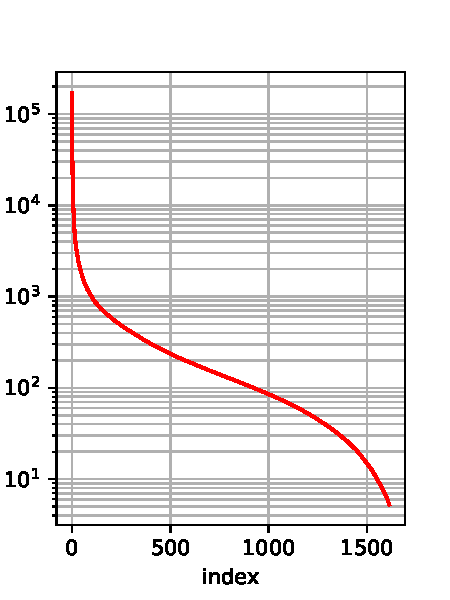
\includegraphics{image/singular_values.pdf}}

    \vspace*{-11em}\hfill
    \begin{tabular}{cccc}
      $r=1$ & $r=2$ & $r=3$ & $r=4$ \\
      \resizebox{0.15\textwidth}{!}{
\includegraphics{image/gray_picture_r1.pdf}} &
      \resizebox{0.15\textwidth}{!}{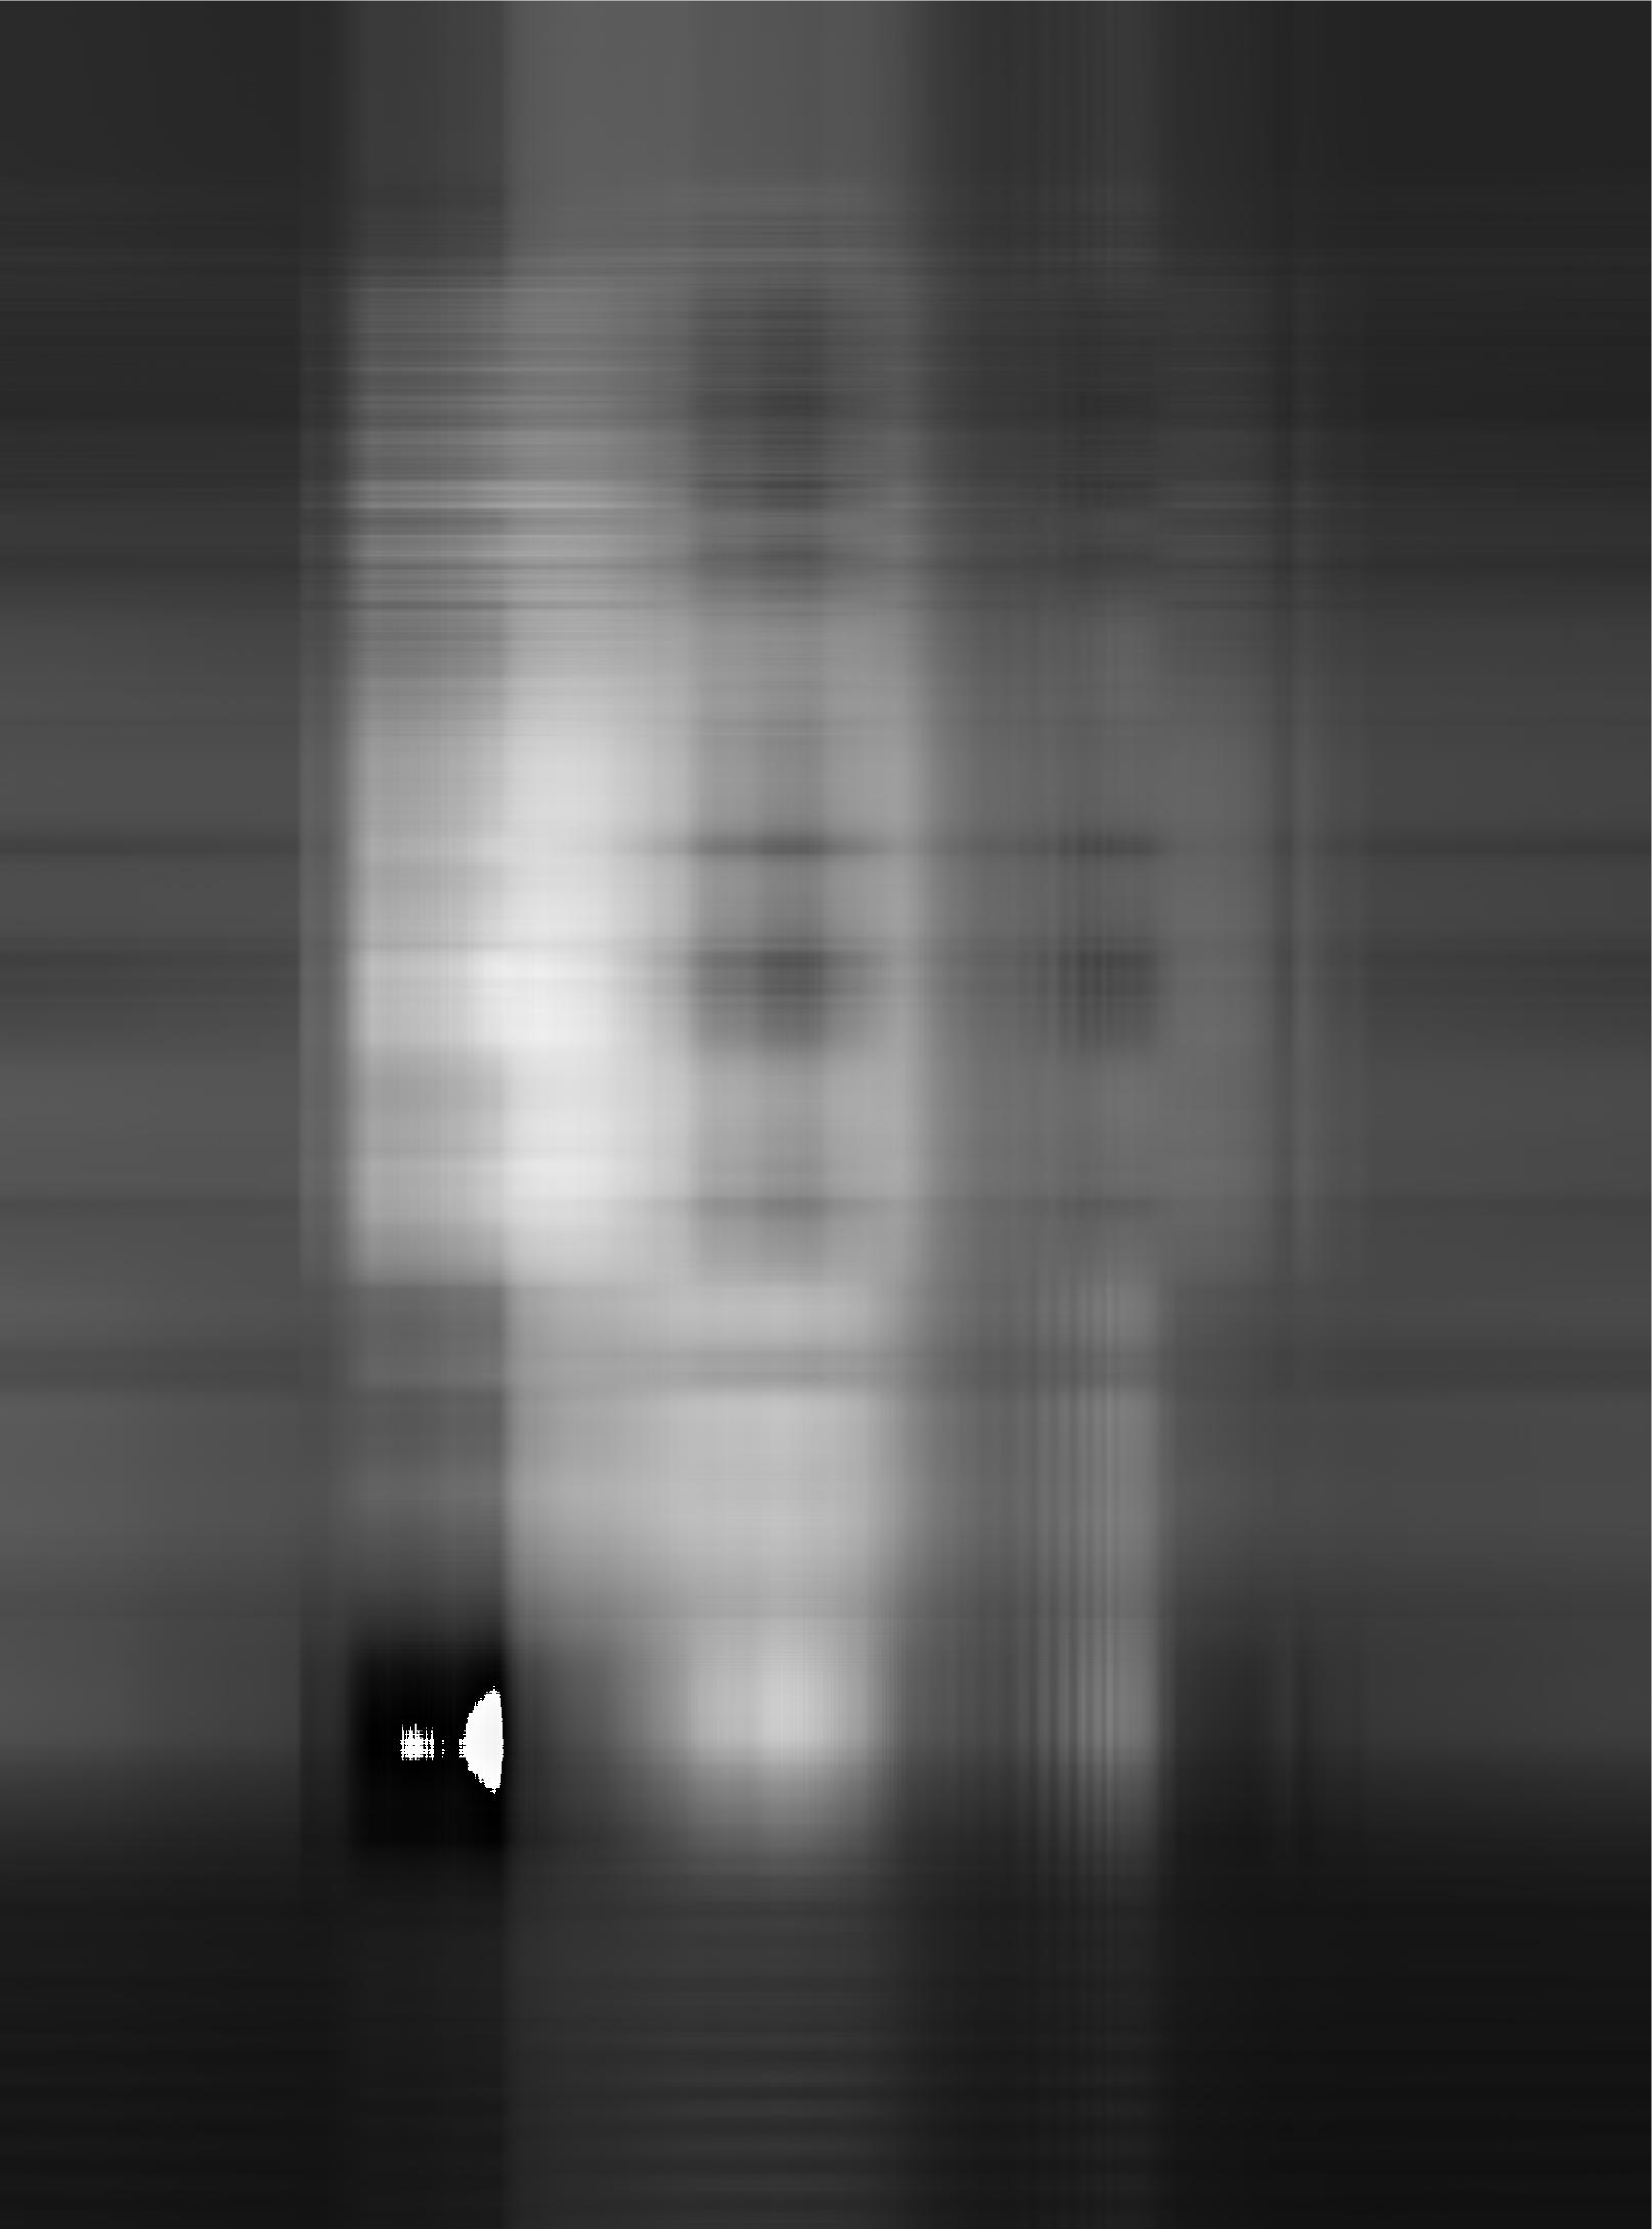
\includegraphics{image/gray_picture_r2.pdf}} &
      \resizebox{0.15\textwidth}{!}{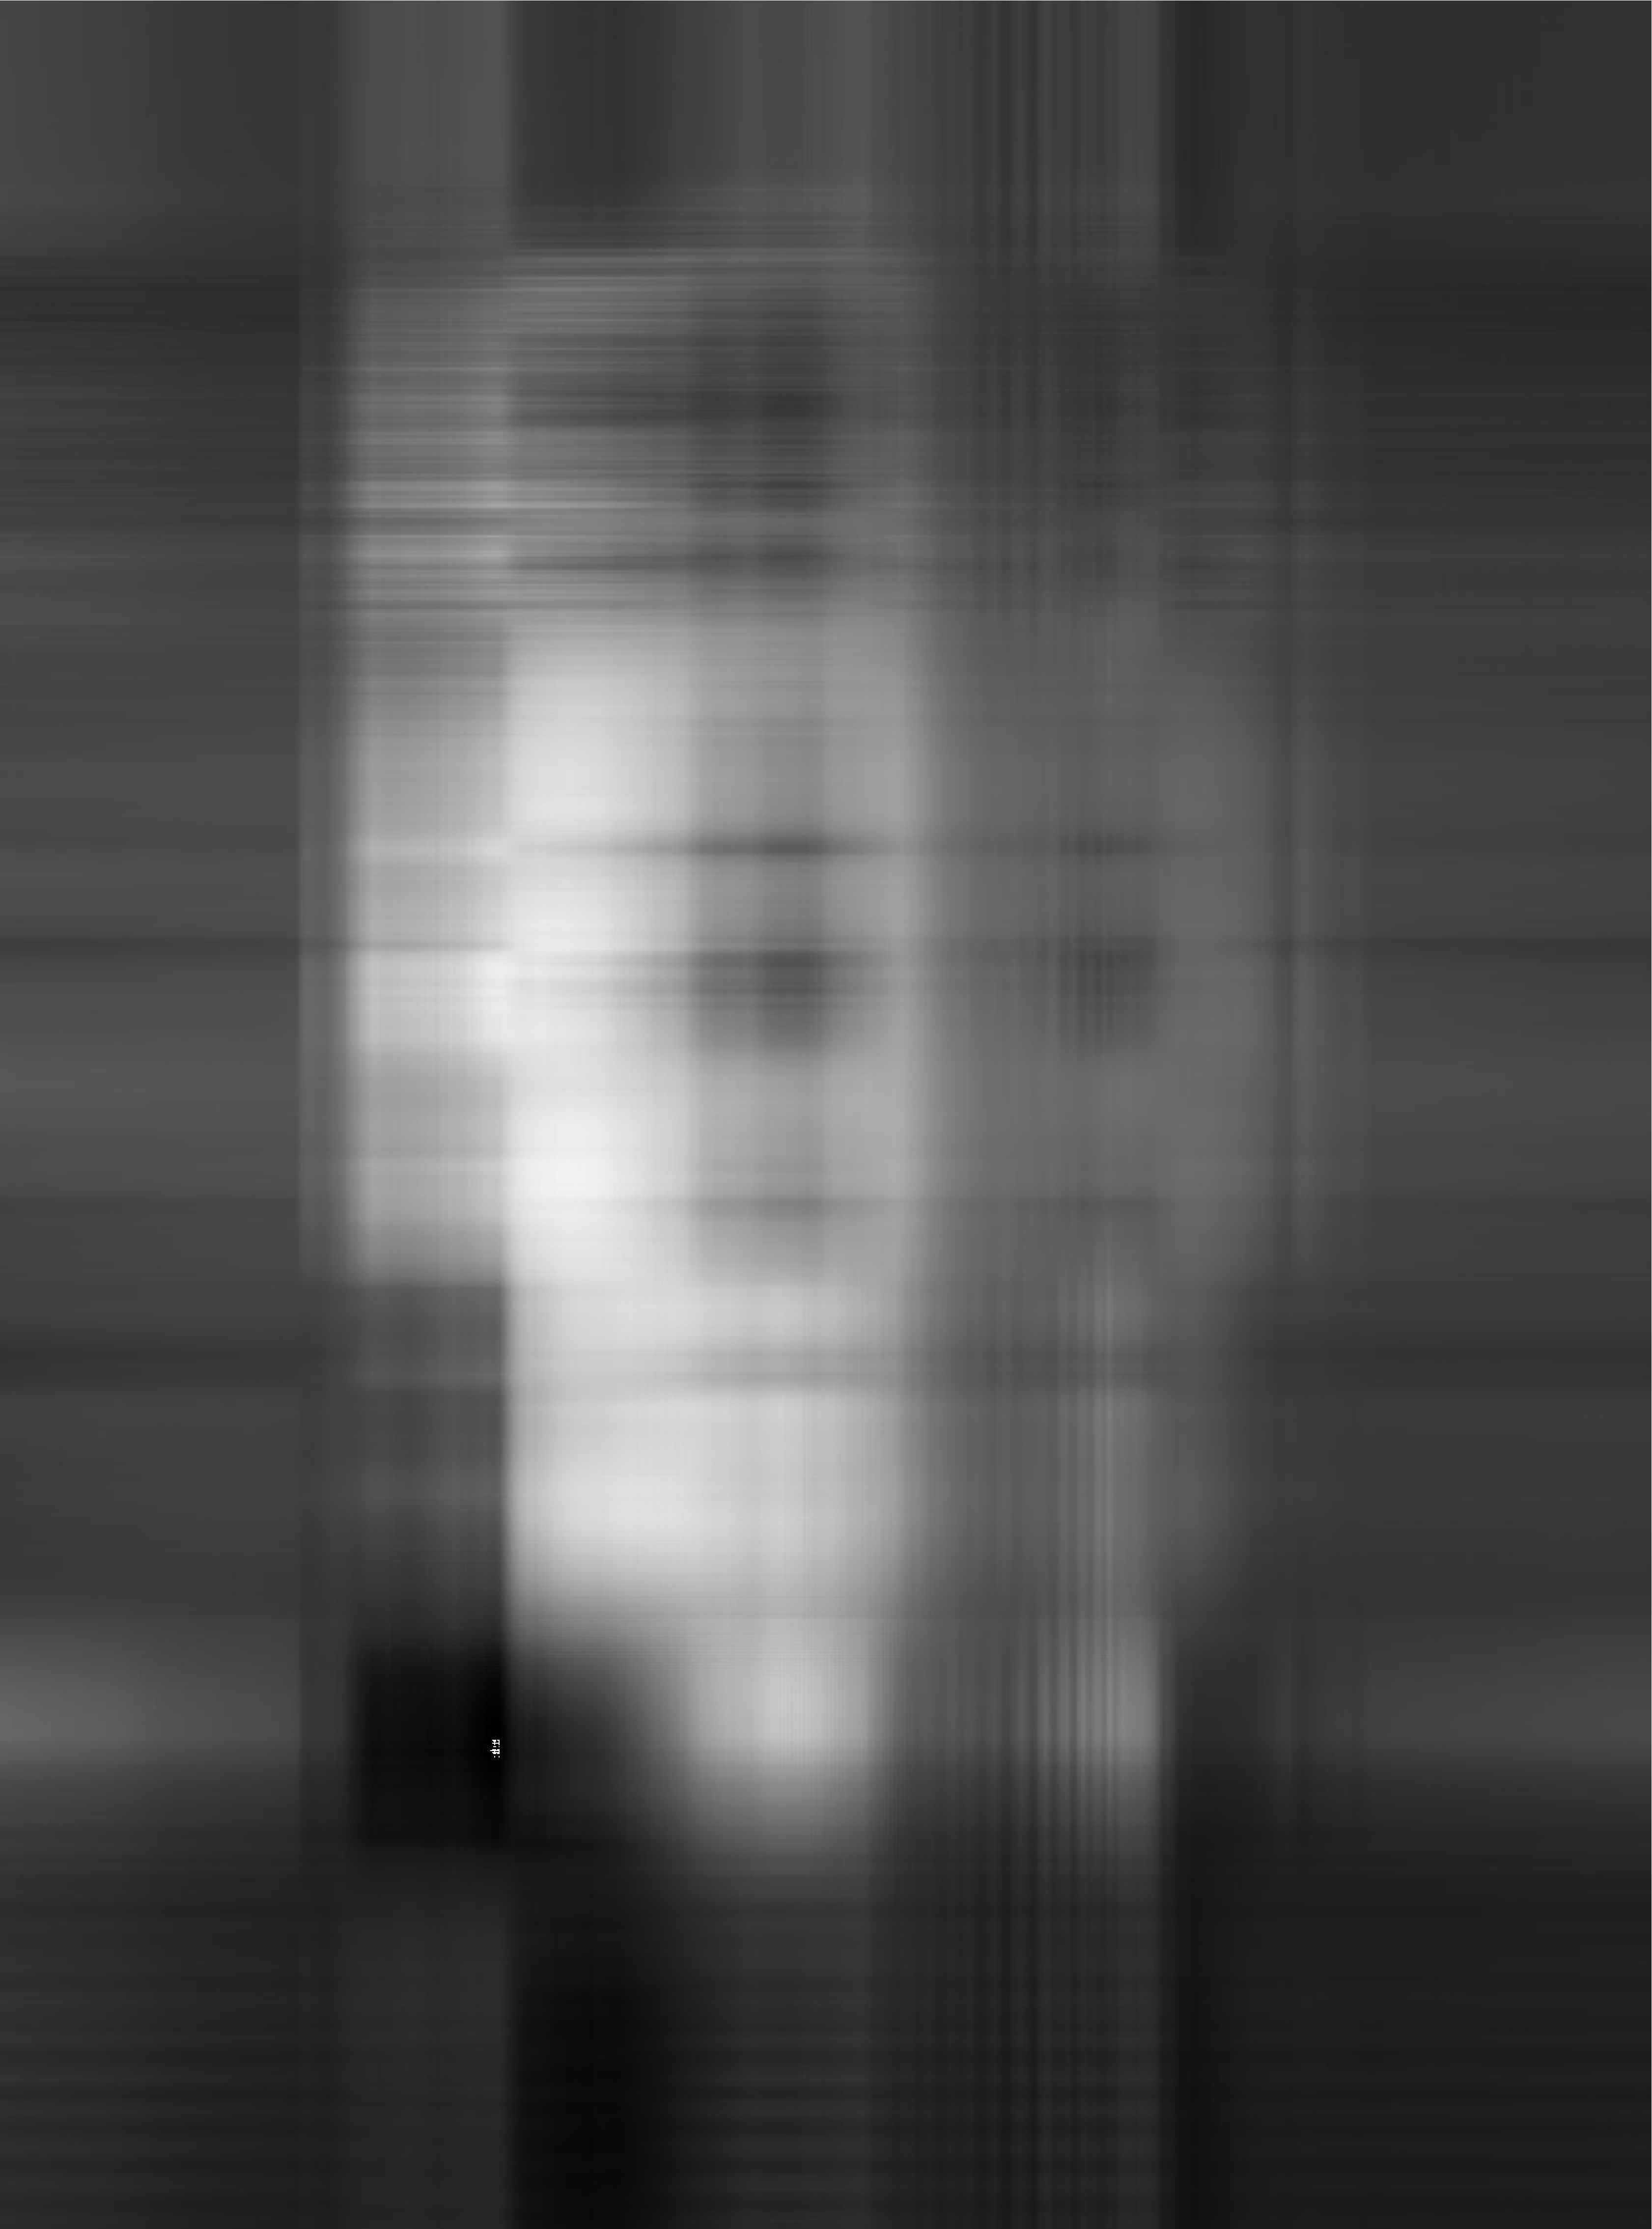
\includegraphics{image/gray_picture_r3.pdf}} &
      \resizebox{0.15\textwidth}{!}{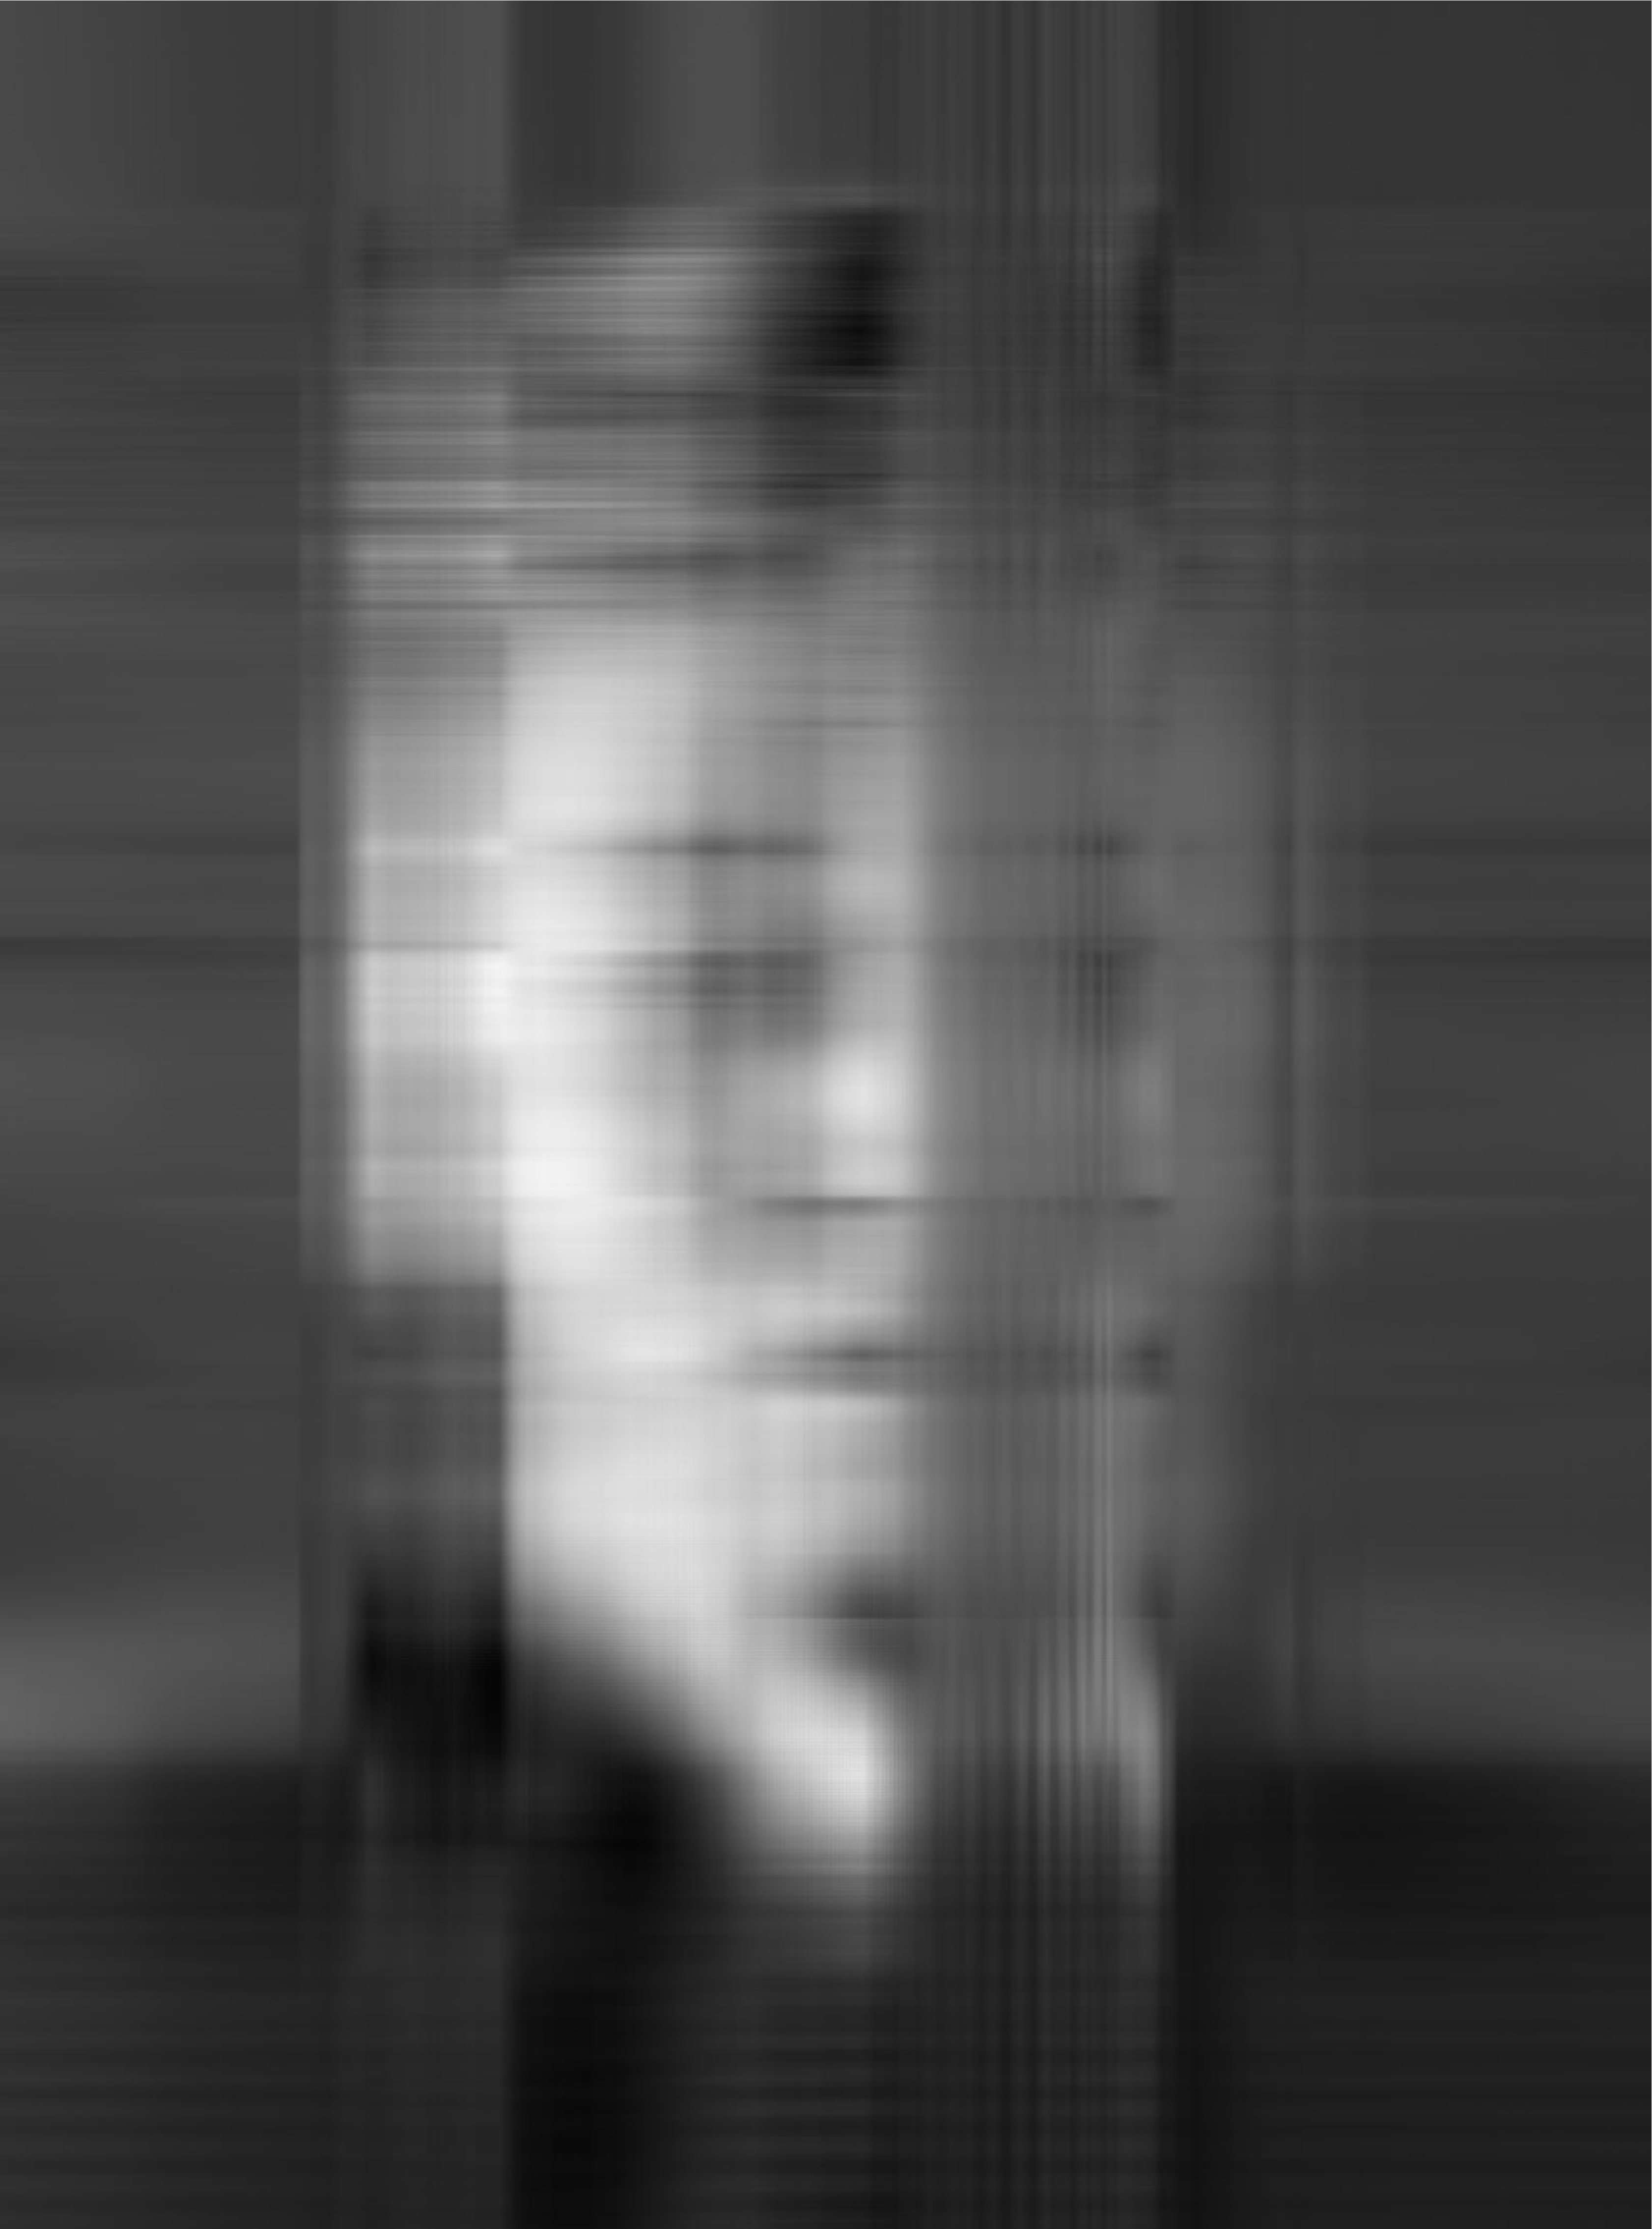
\includegraphics{image/gray_picture_r4.pdf}} \\
    \end{tabular}
  \end{itemize}
\end{frame}

\begin{frame}[t,fragile]{特異値分解による画像圧縮}
  \begin{itemize}
  \item 特異値の分布とランク$r$近似 ($1614 \times 2178$グレイスケール写真)
    
    \hspace*{-3em}\resizebox{0.27\textwidth}{!}{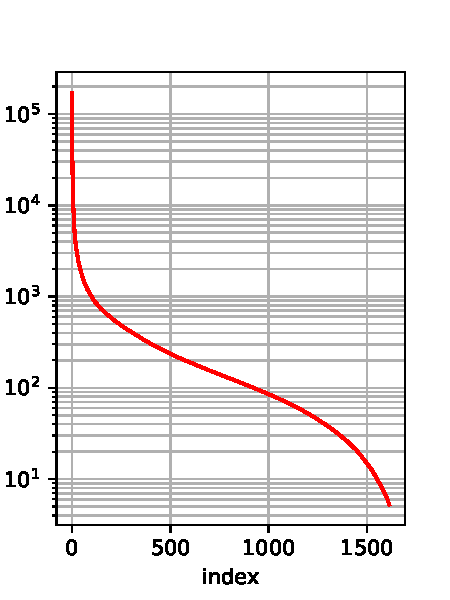
\includegraphics{image/singular_values.pdf}}

    \vspace*{-11em}\hfill
    \begin{tabular}{cccc}
      $r=1$ & $r=2$ & $r=3$ & $r=4$ \\
      \resizebox{0.15\textwidth}{!}{
\includegraphics{image/gray_picture_r1.pdf}} &
      \resizebox{0.15\textwidth}{!}{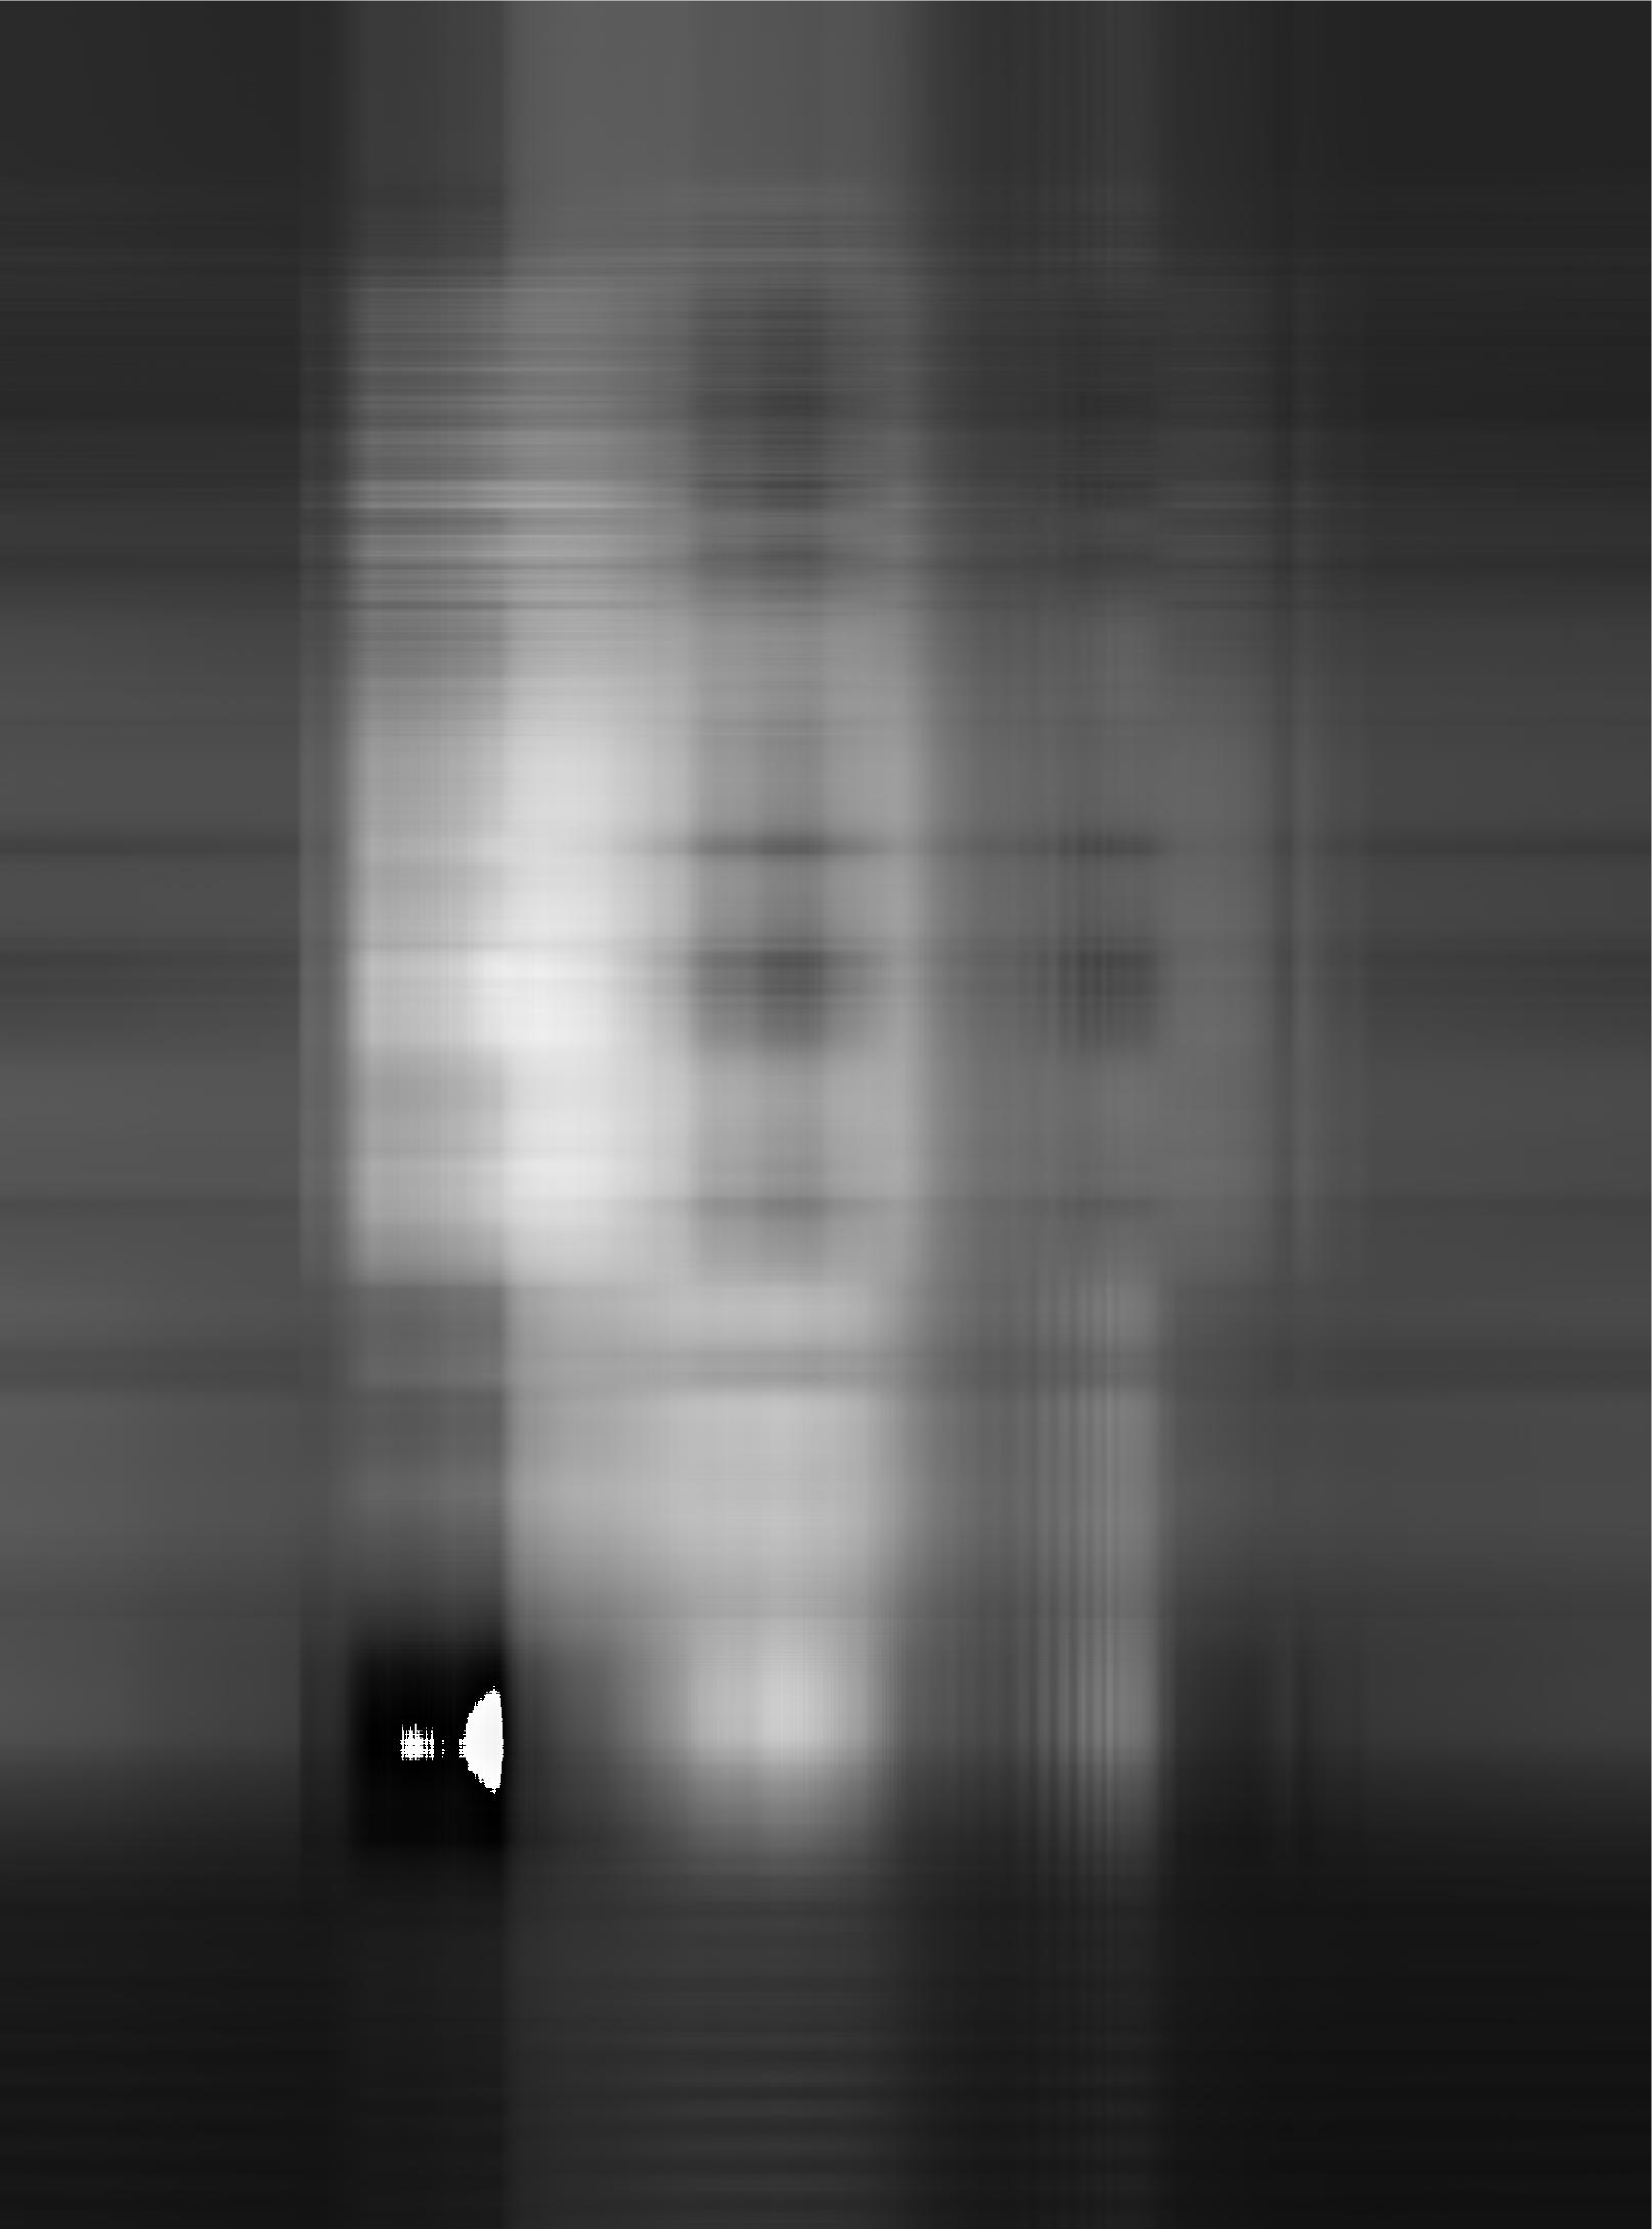
\includegraphics{image/gray_picture_r2.pdf}} &
      \resizebox{0.15\textwidth}{!}{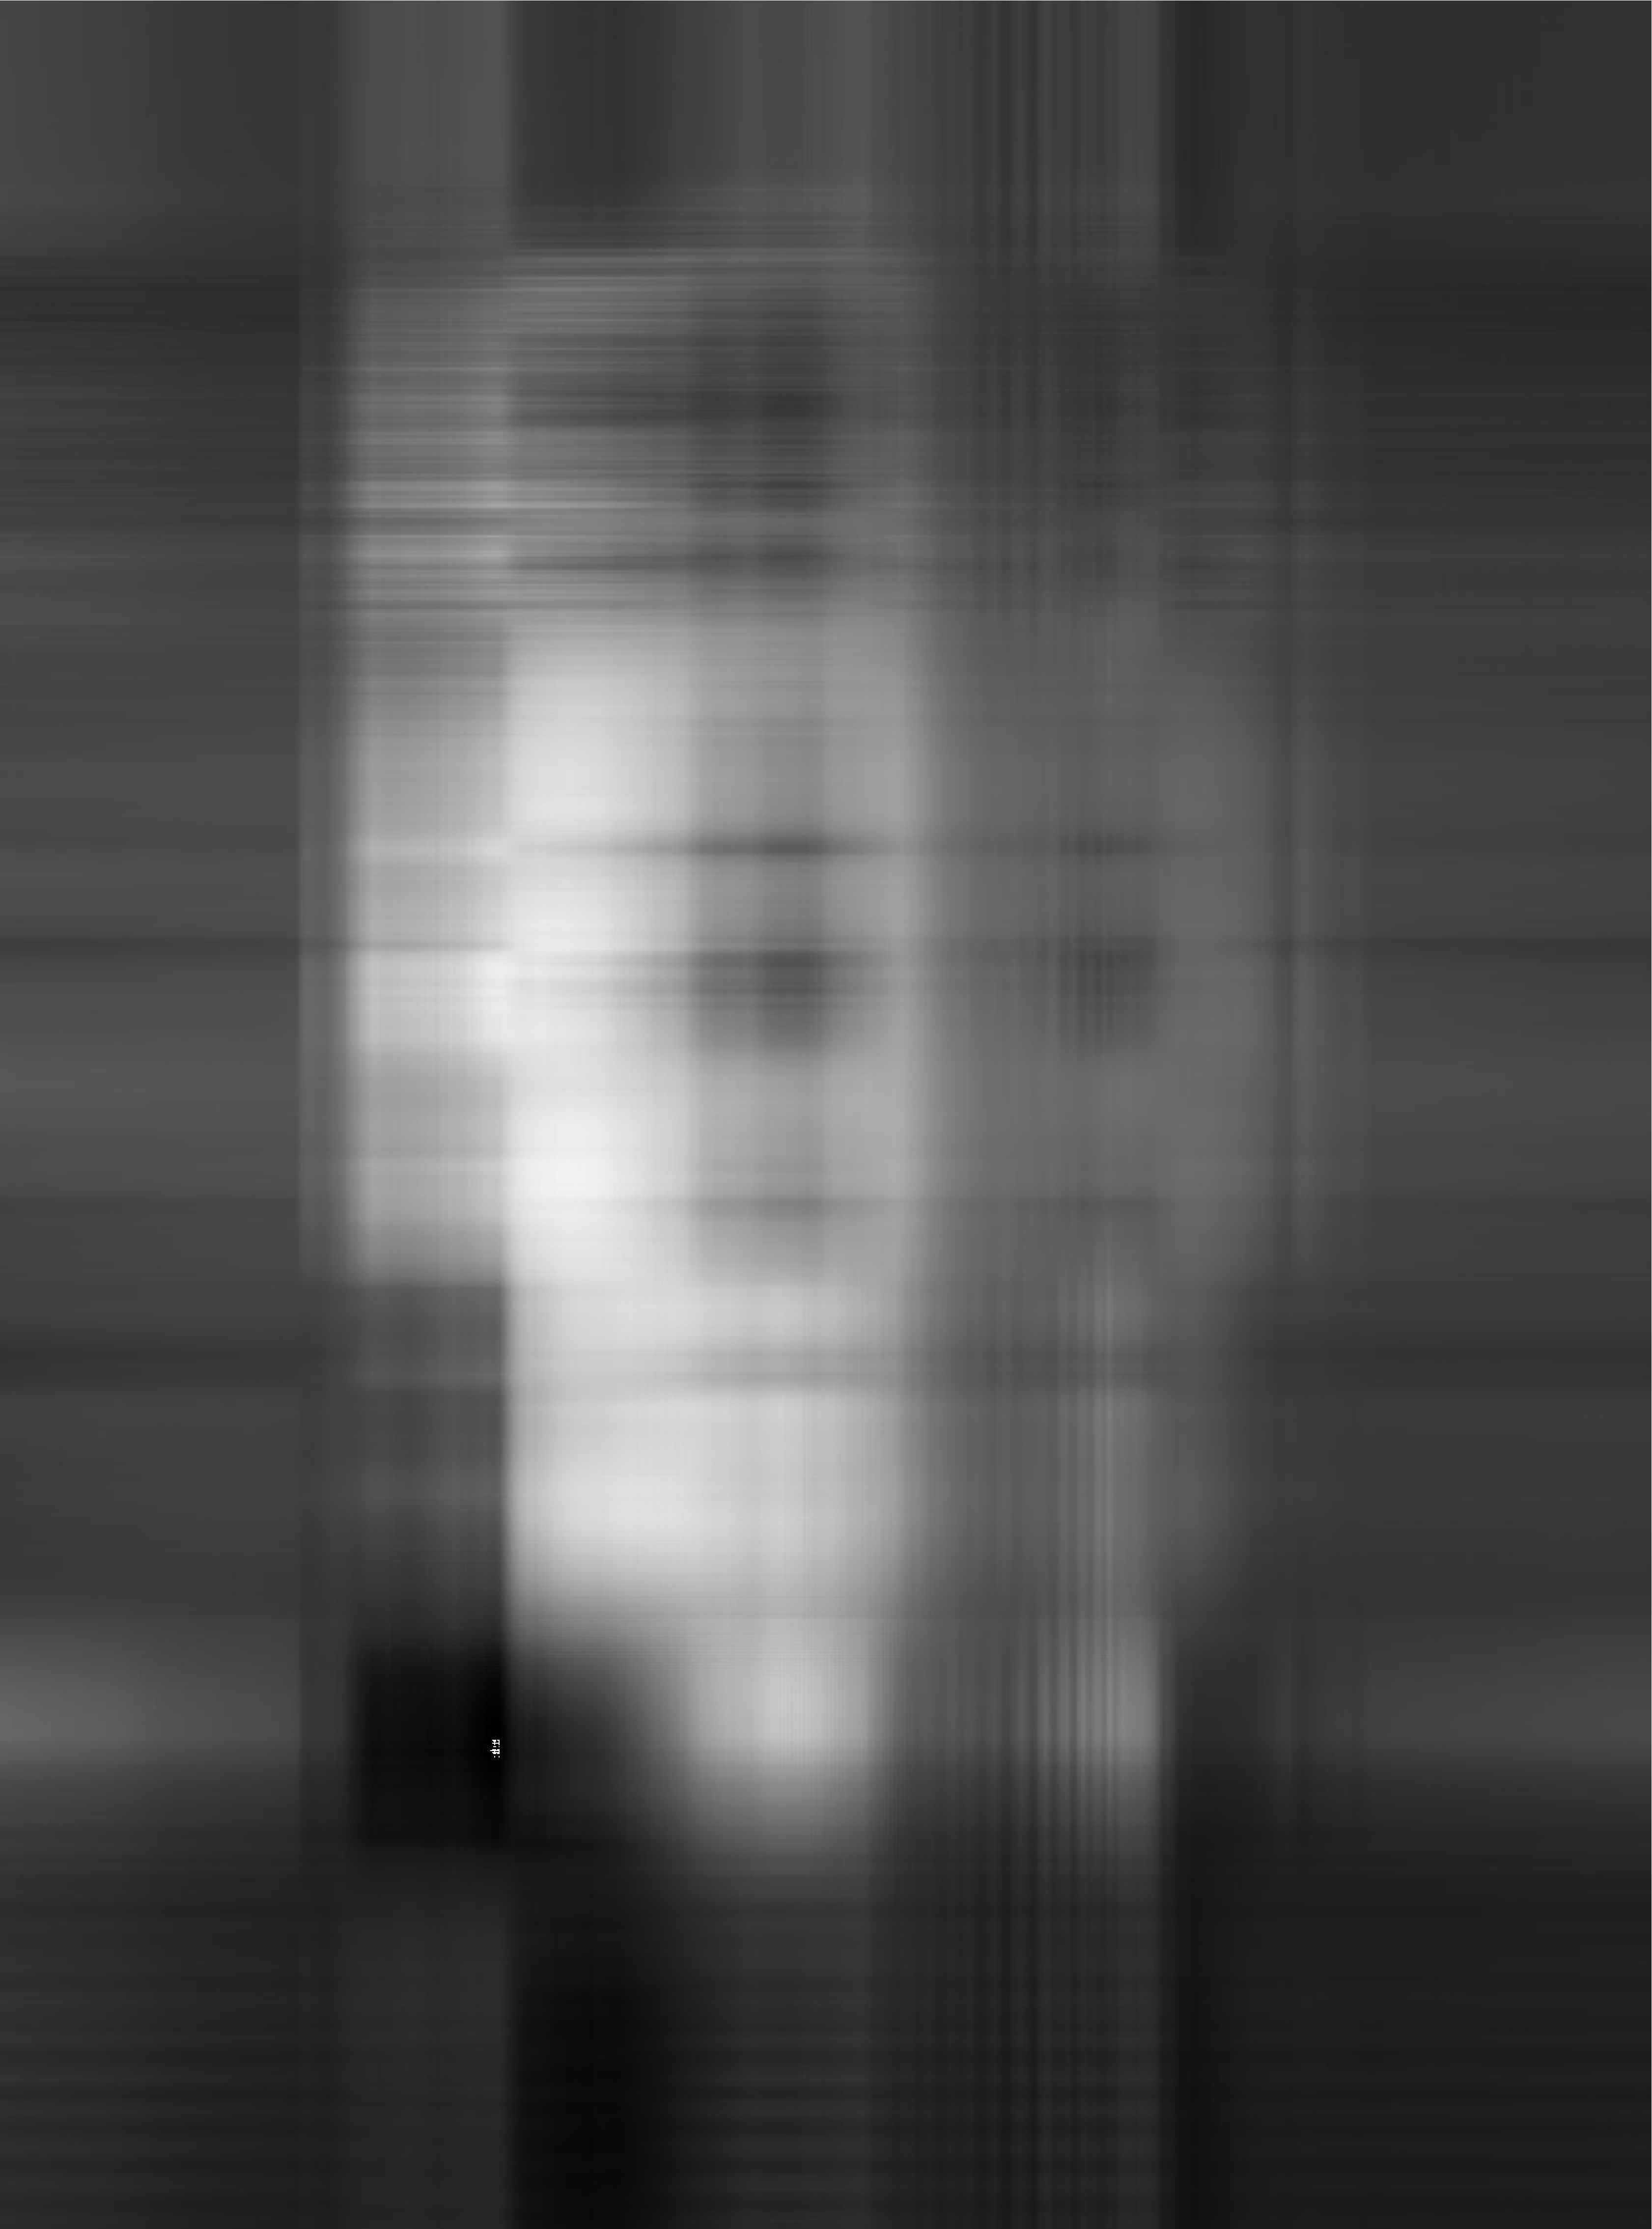
\includegraphics{image/gray_picture_r3.pdf}} &
      \resizebox{0.15\textwidth}{!}{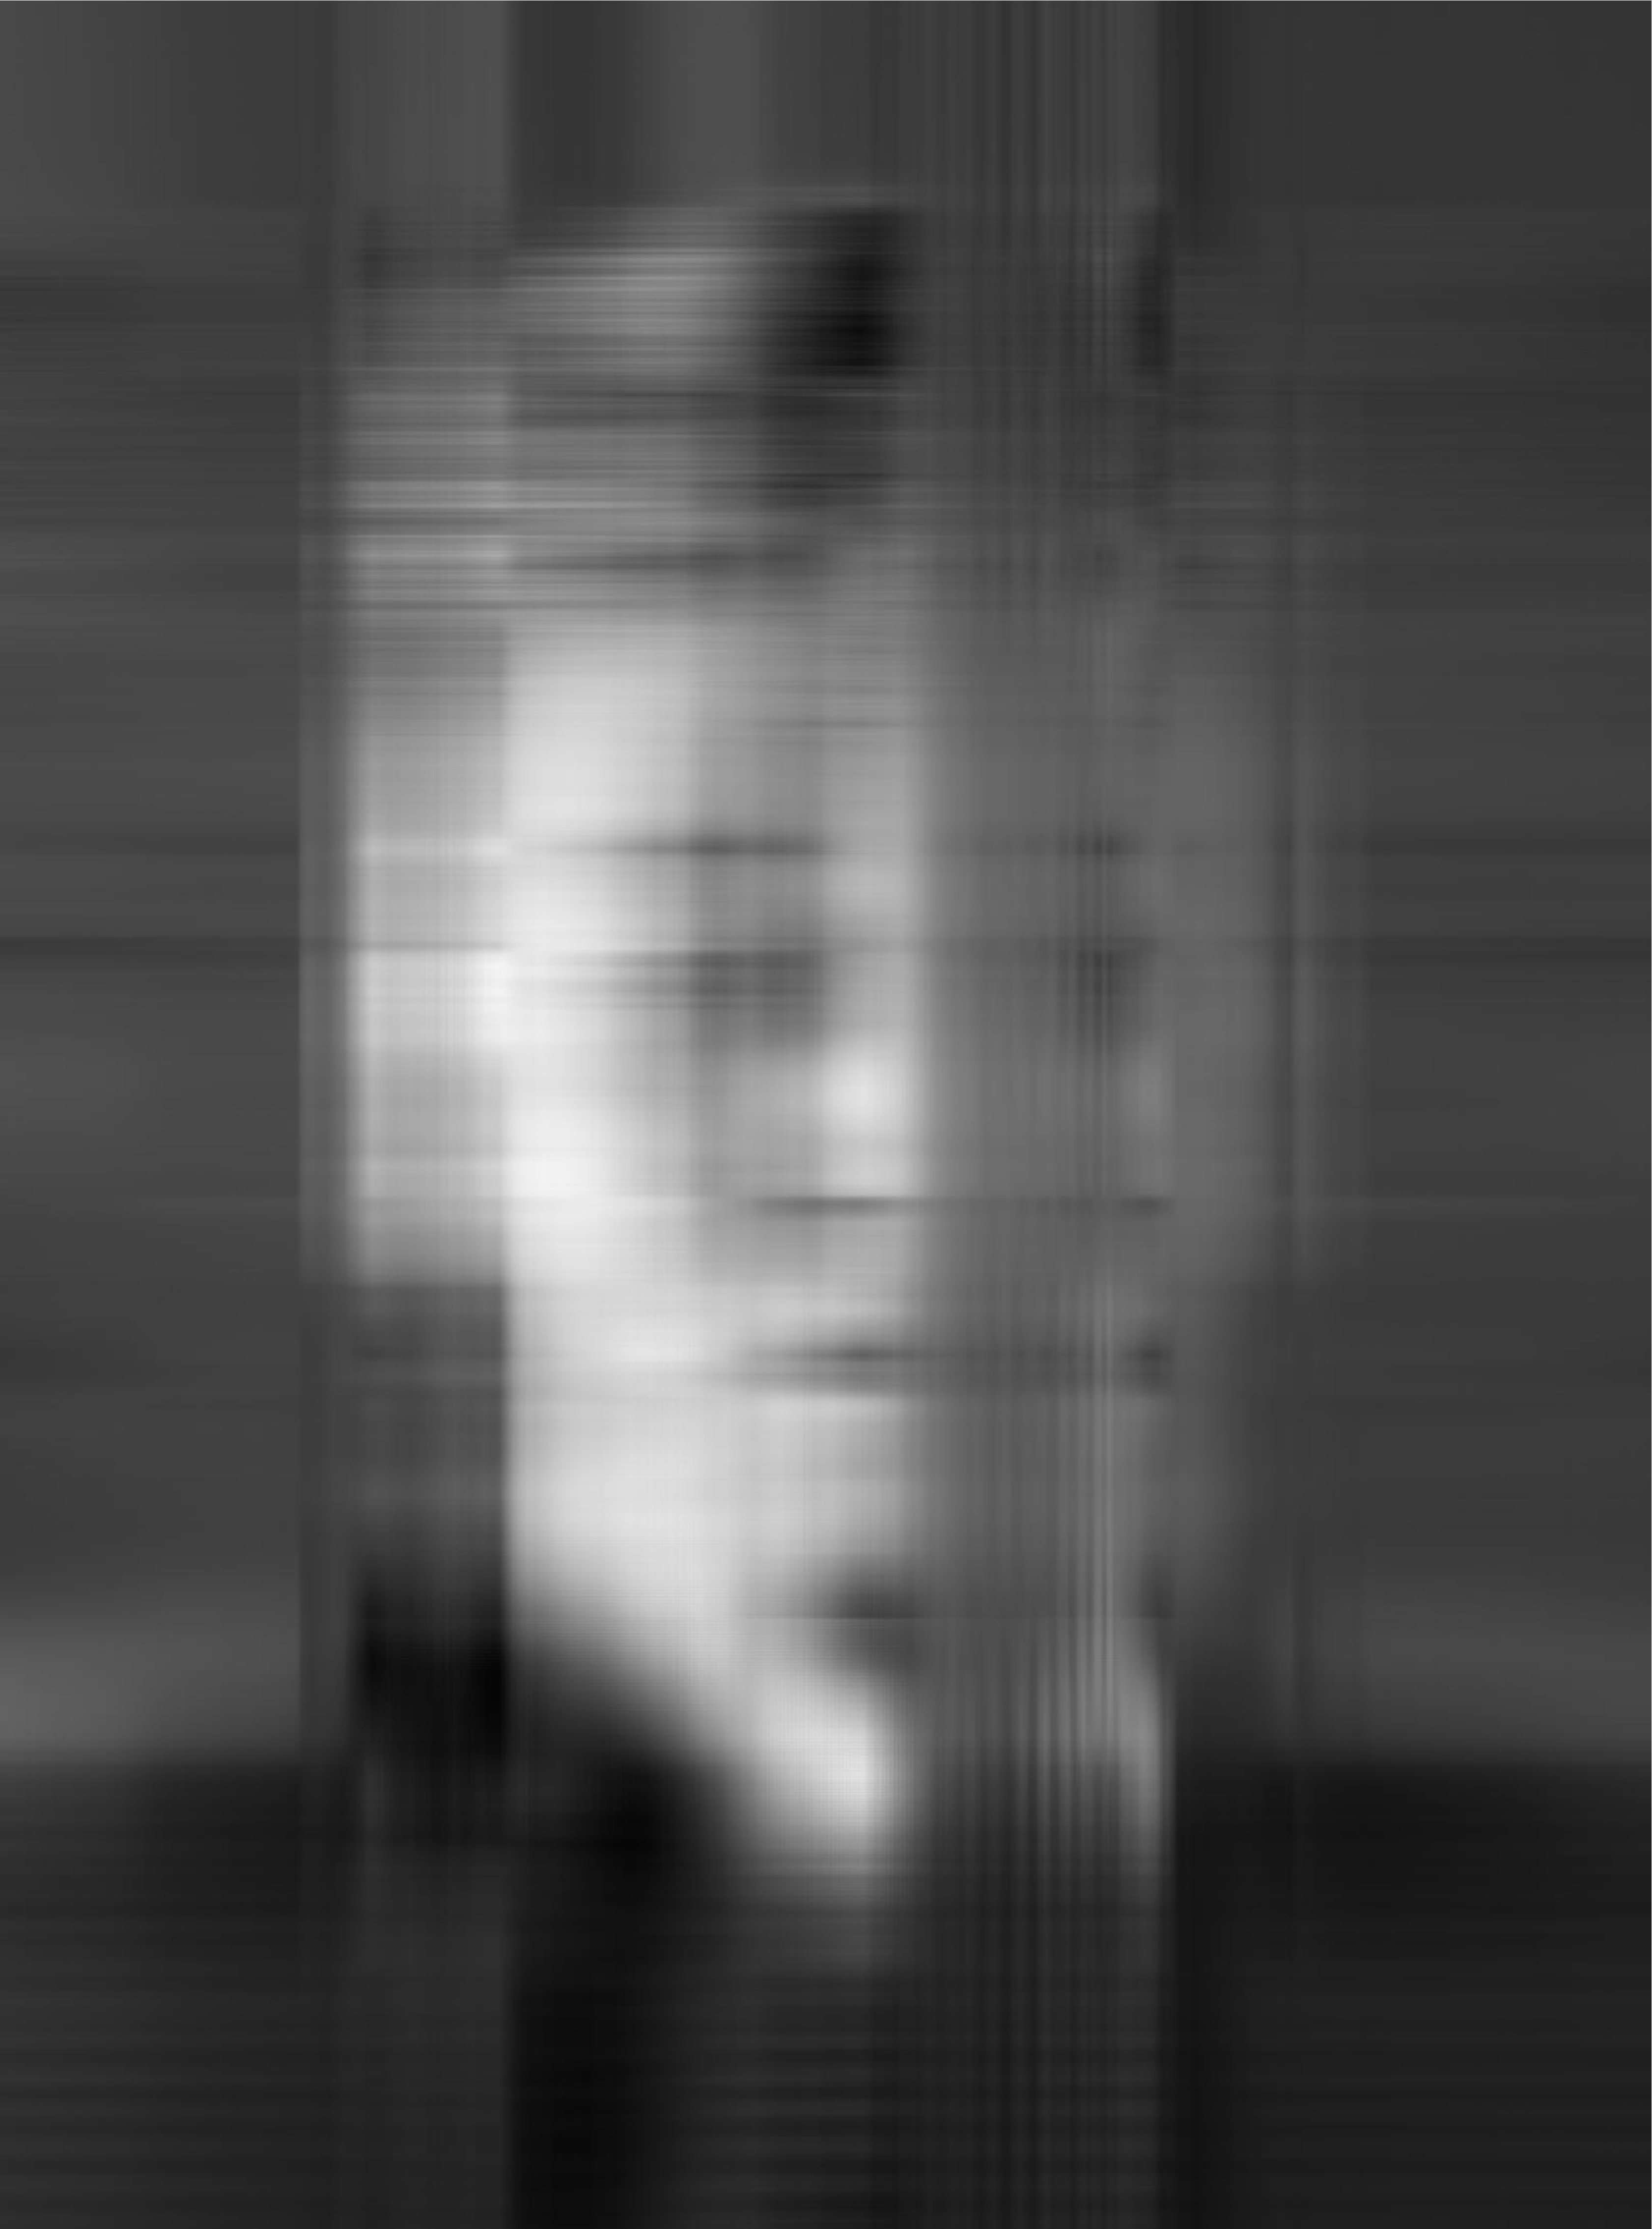
\includegraphics{image/gray_picture_r4.pdf}} \\
      $r=5$ & $r=10$ & $r=20$ & $r=50$ \\
      \resizebox{0.15\textwidth}{!}{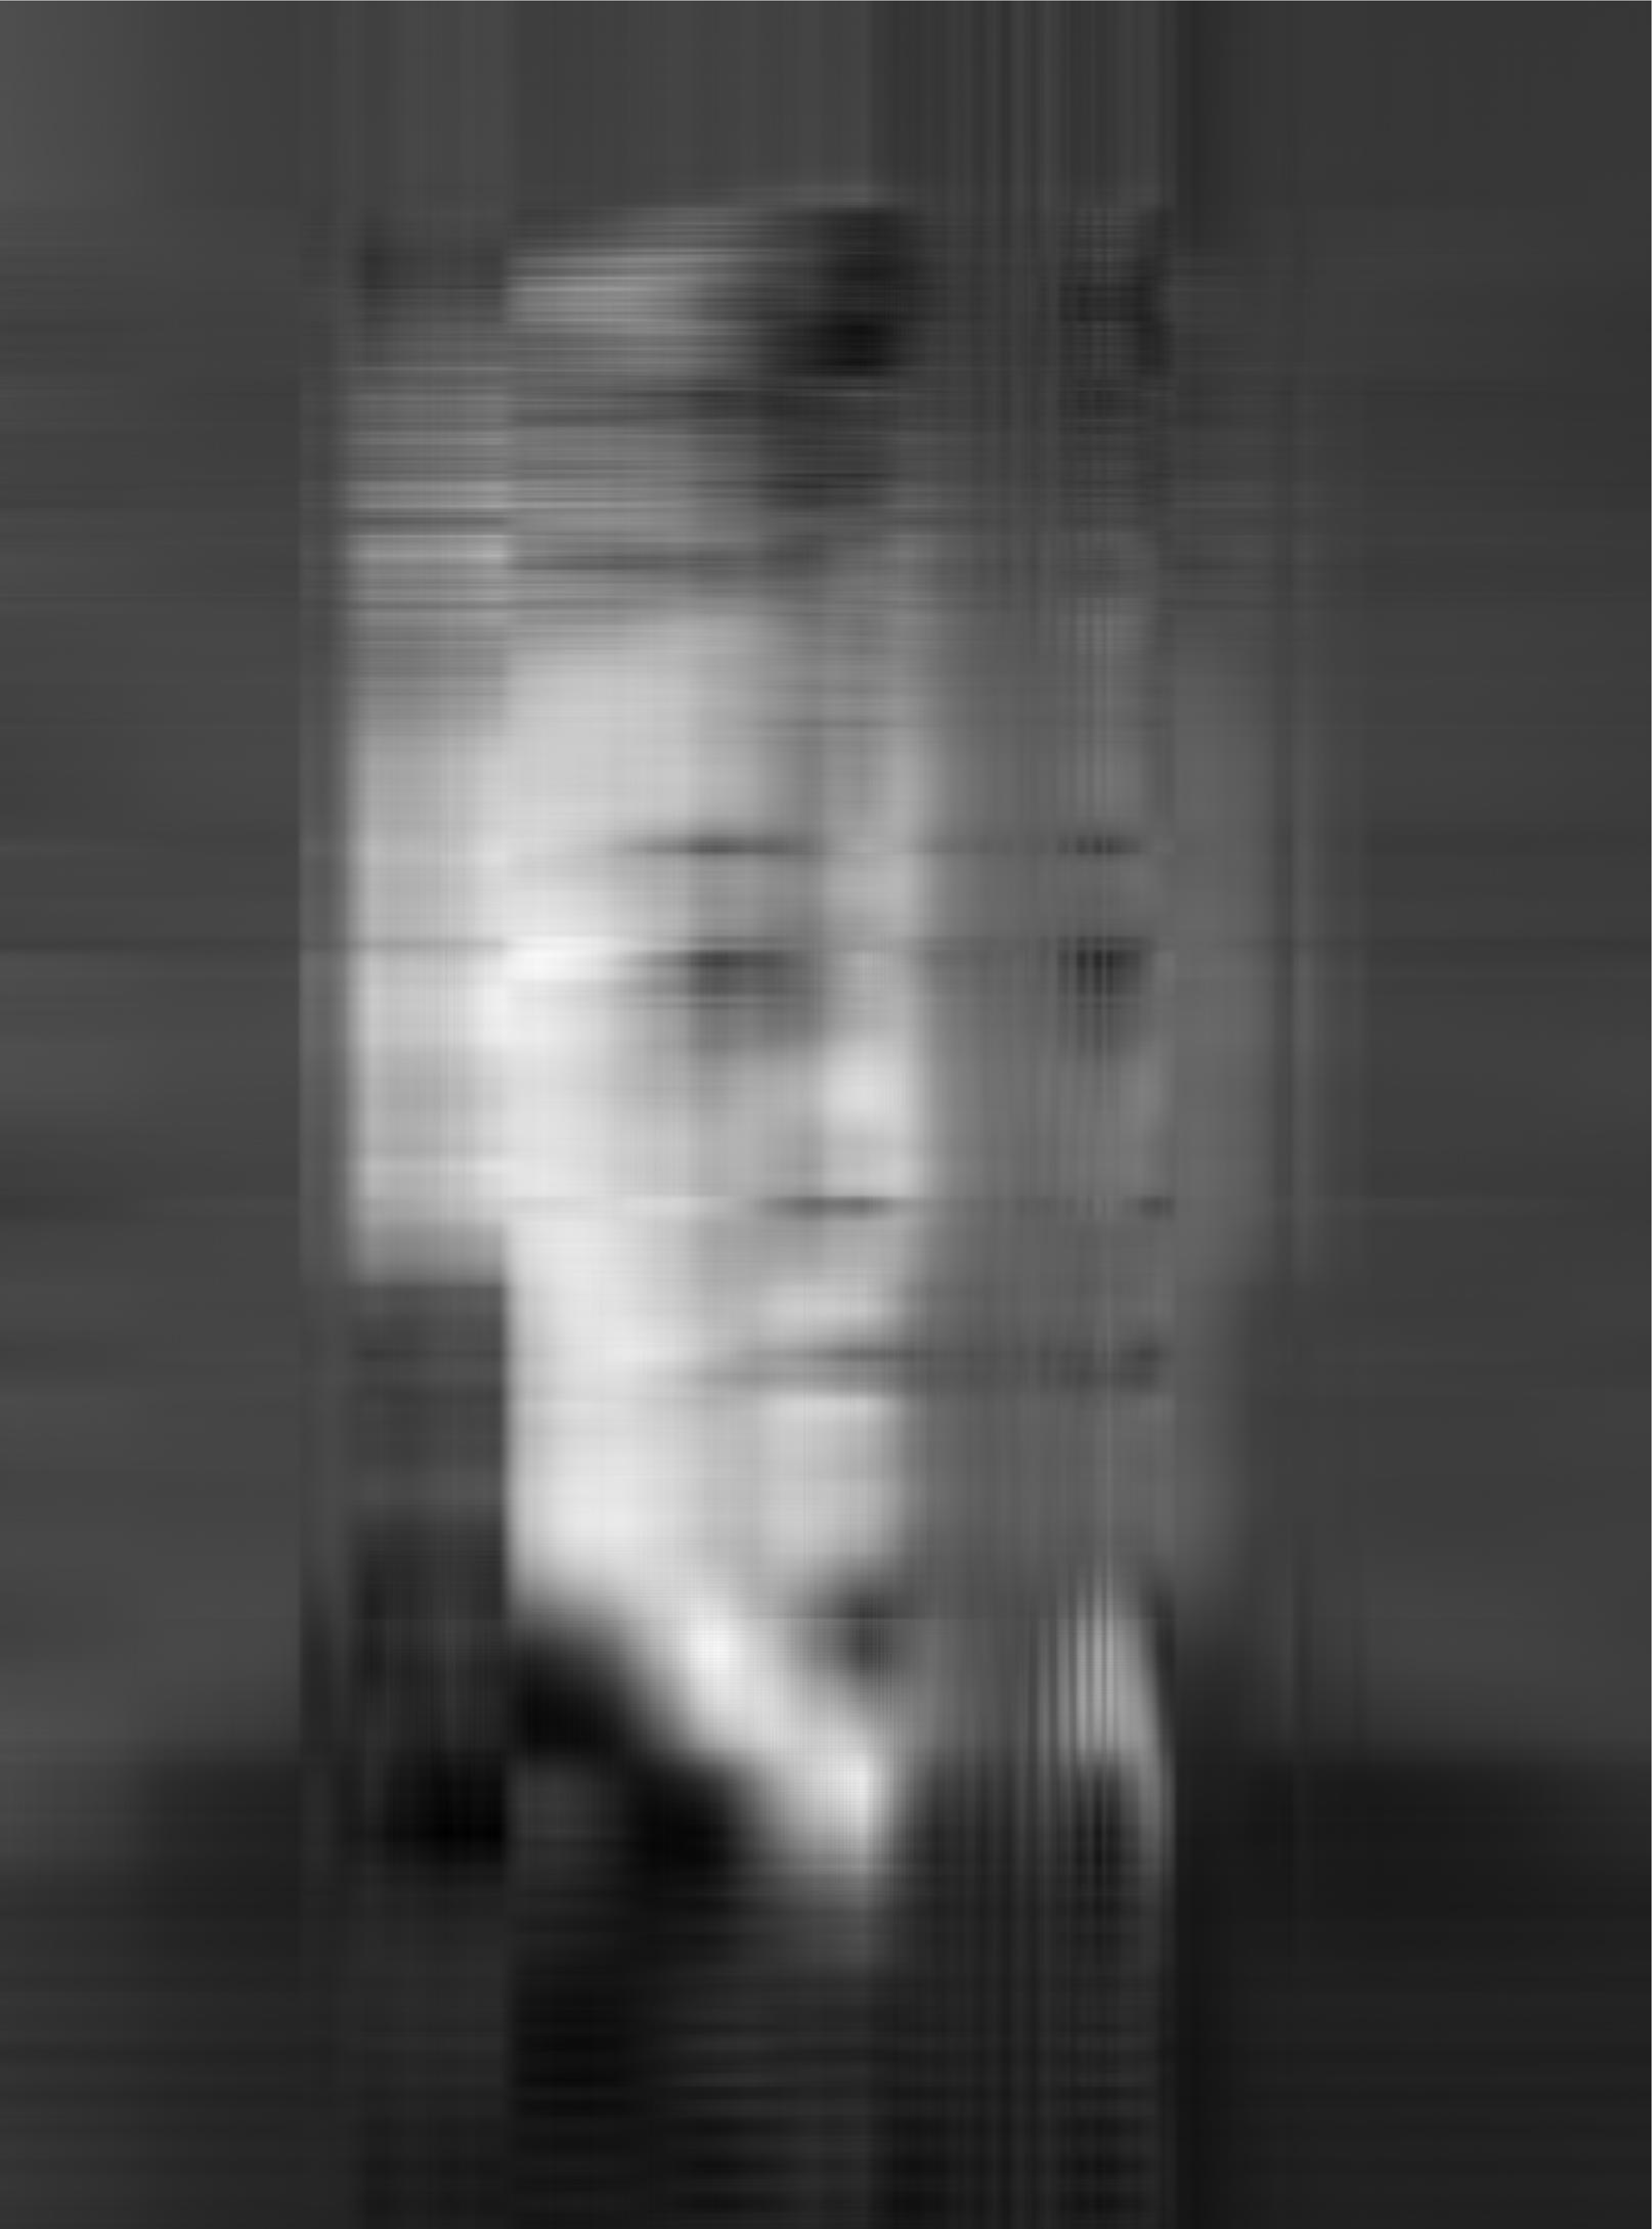
\includegraphics{image/gray_picture_r5.pdf}} &
      \resizebox{0.15\textwidth}{!}{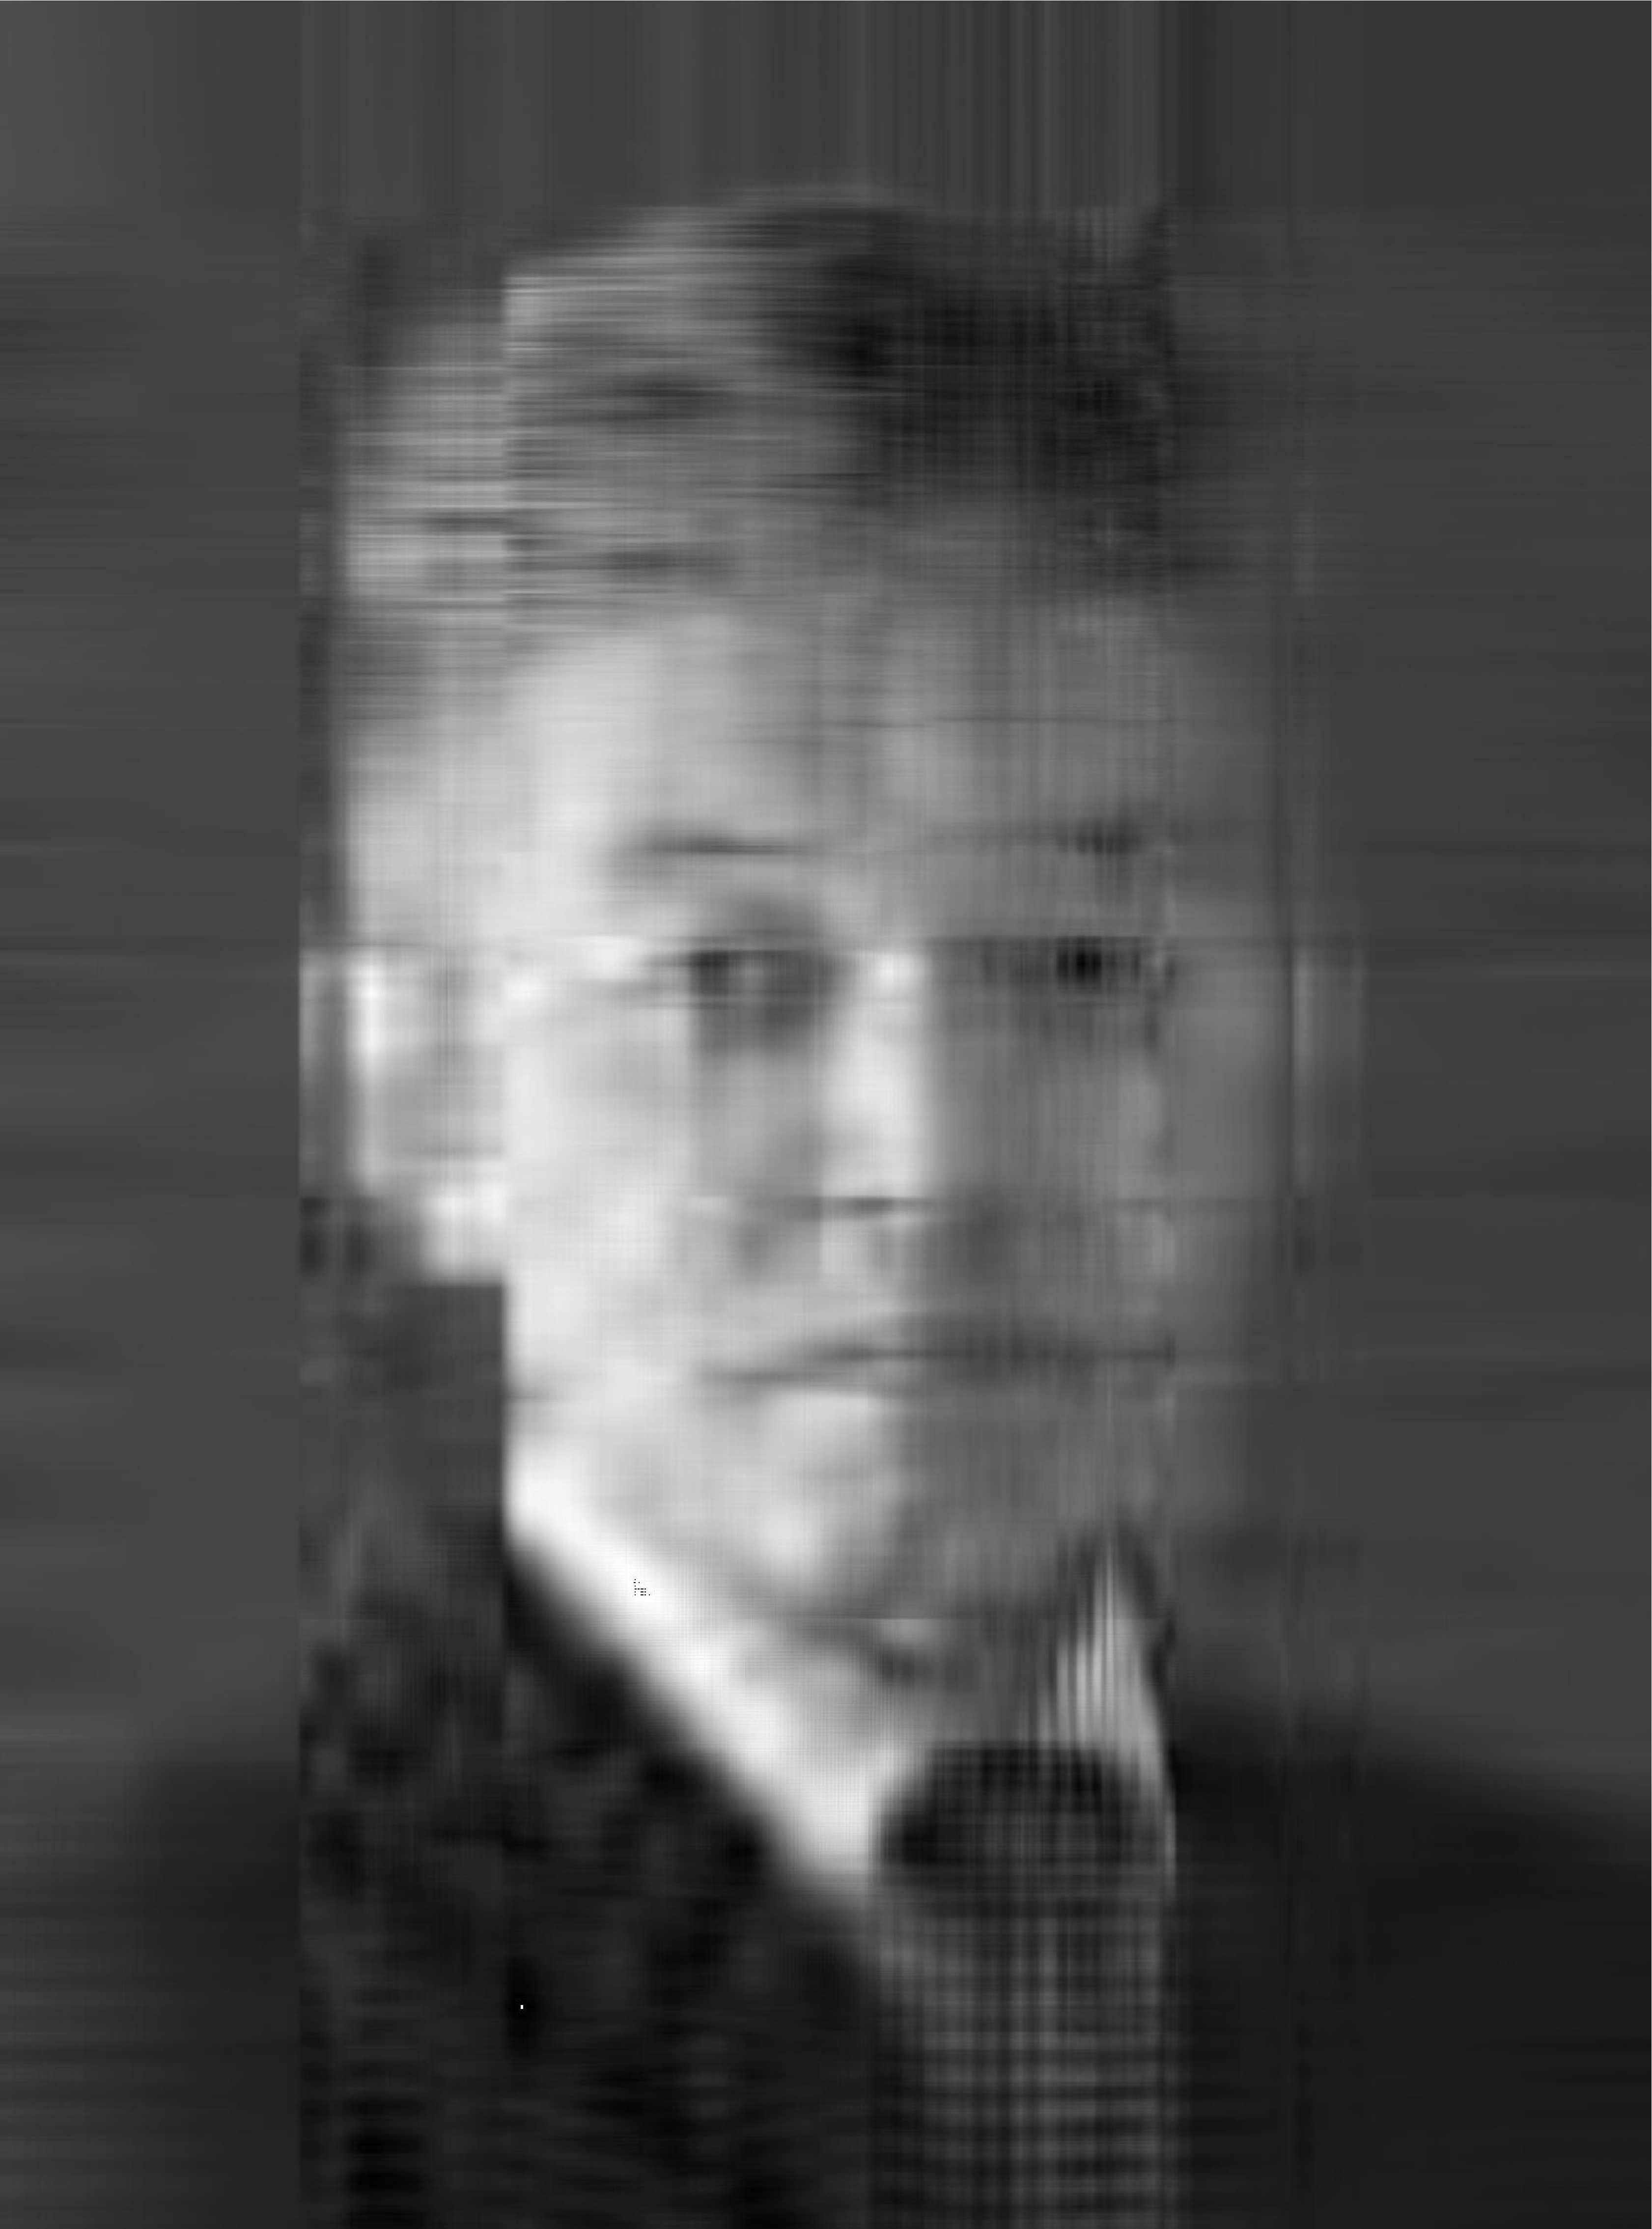
\includegraphics{image/gray_picture_r10.pdf}} &
      \resizebox{0.15\textwidth}{!}{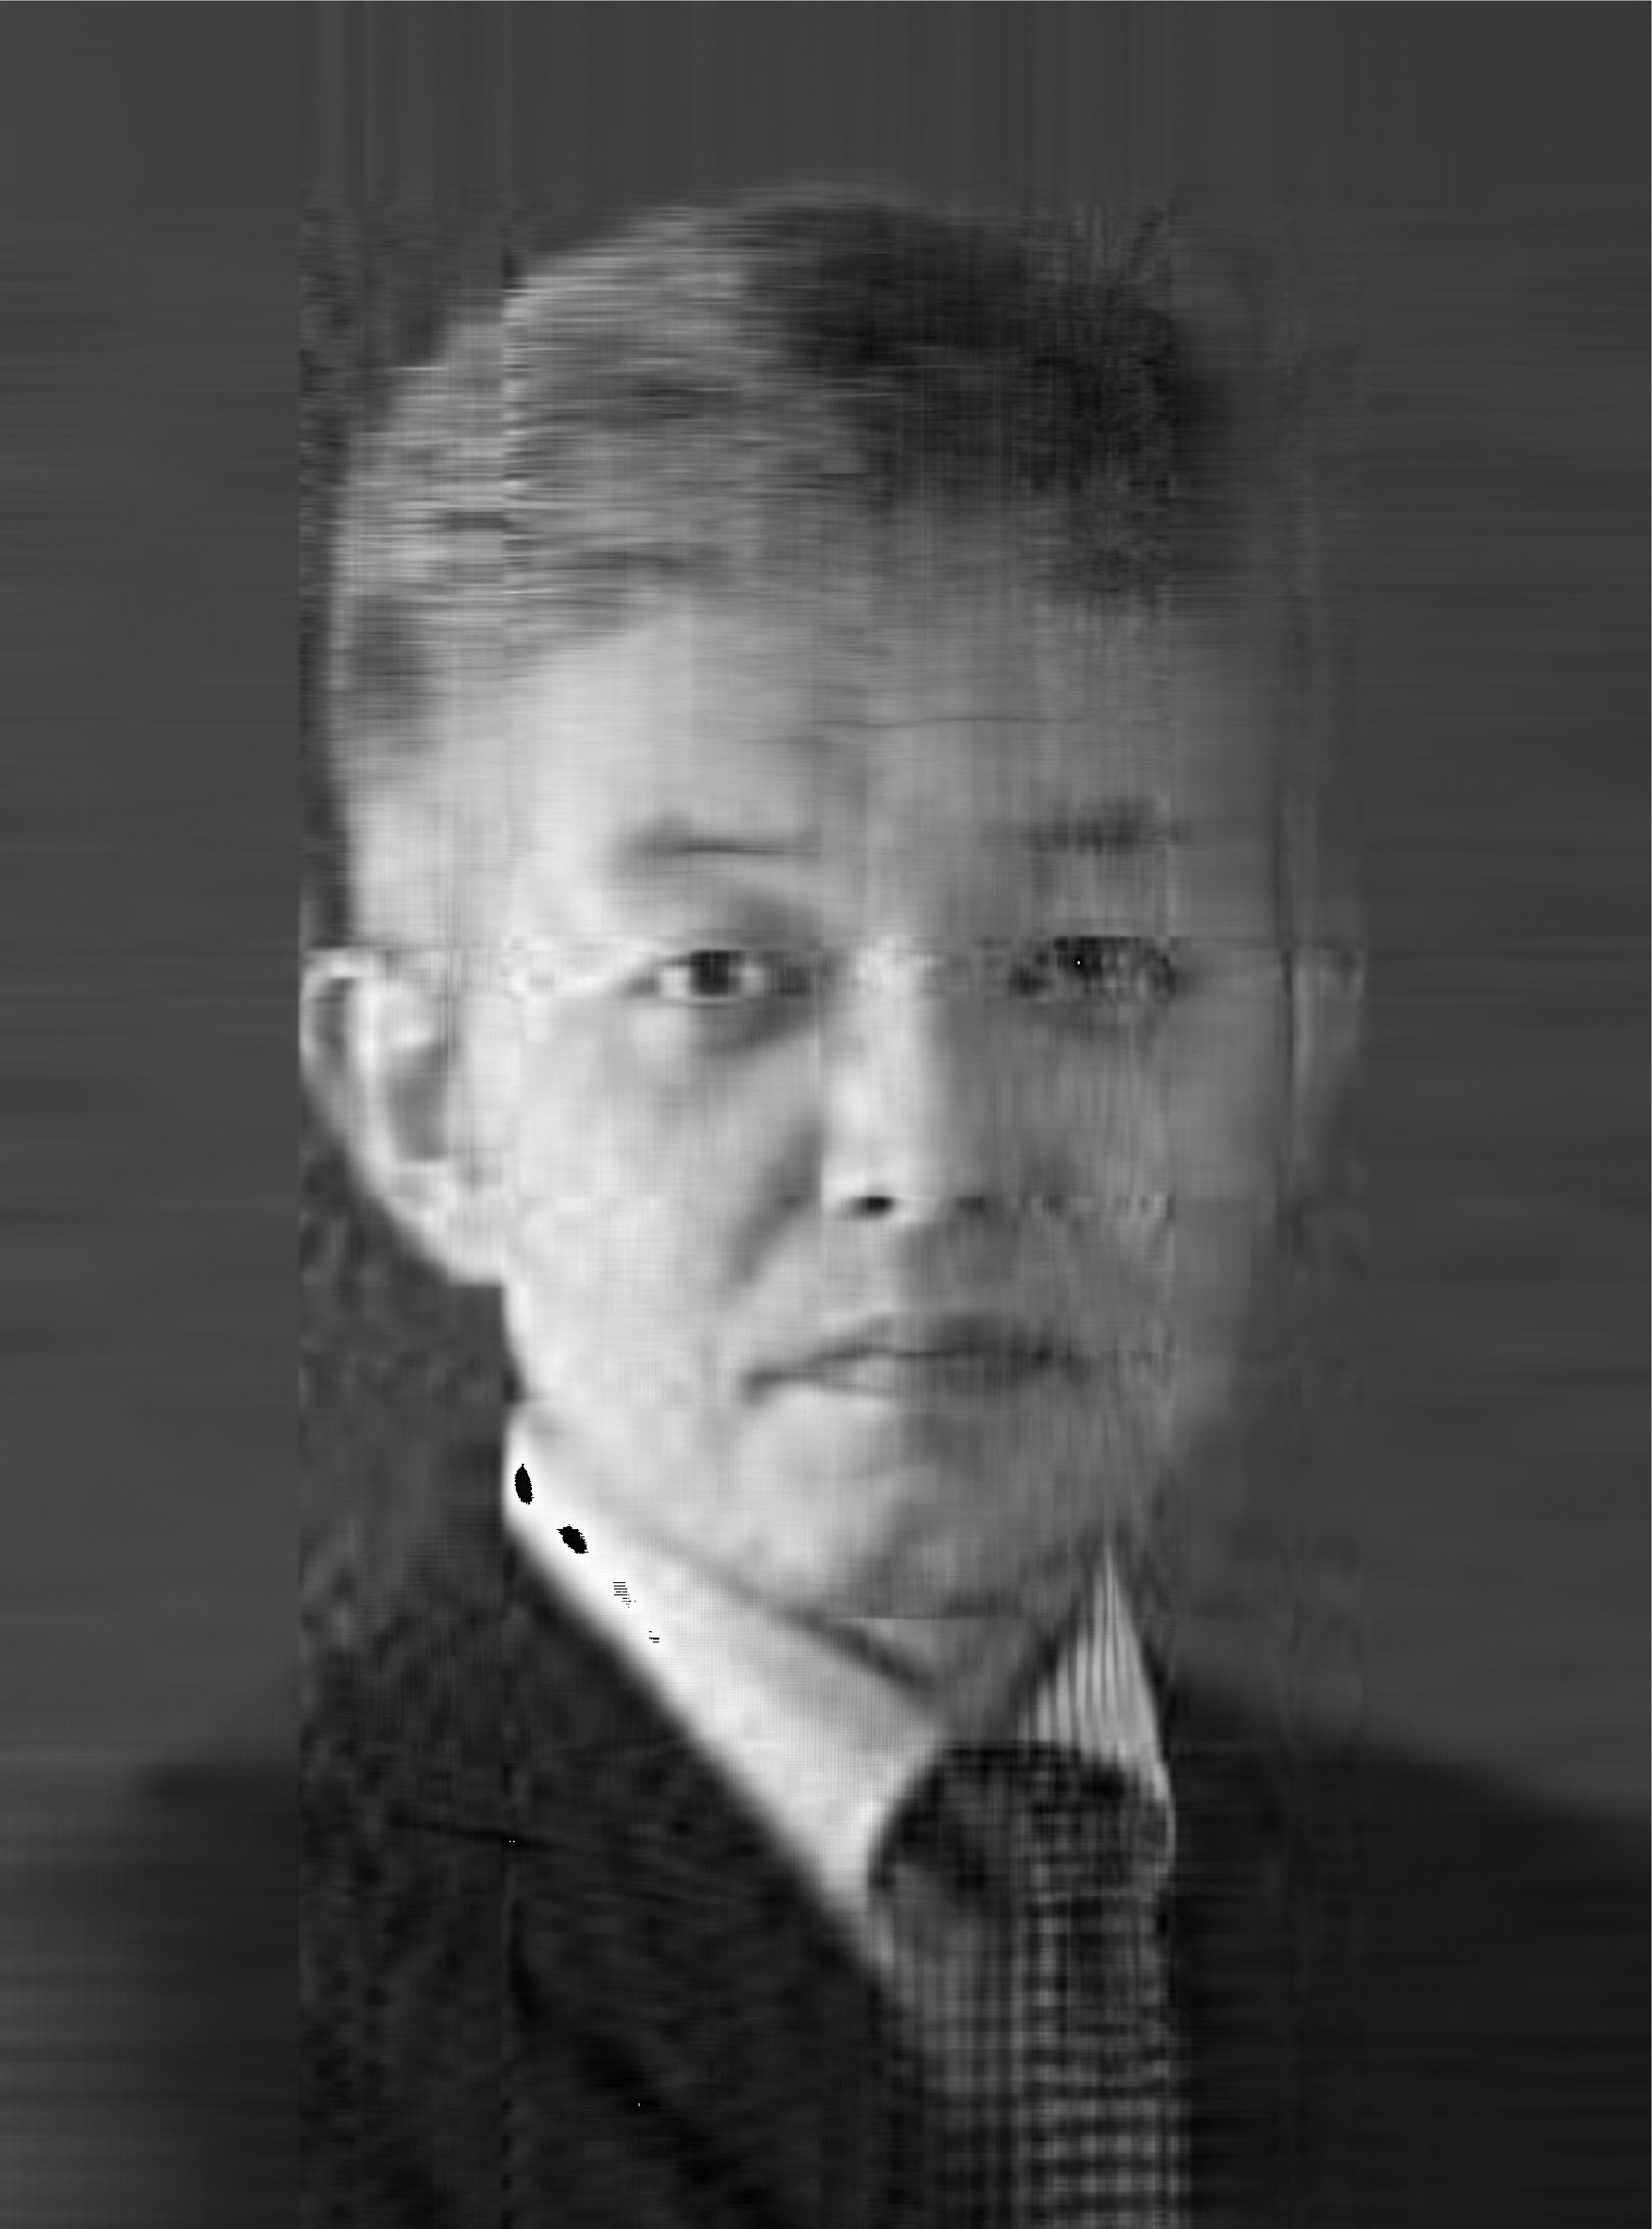
\includegraphics{image/gray_picture_r20.pdf}} &
      \resizebox{0.15\textwidth}{!}{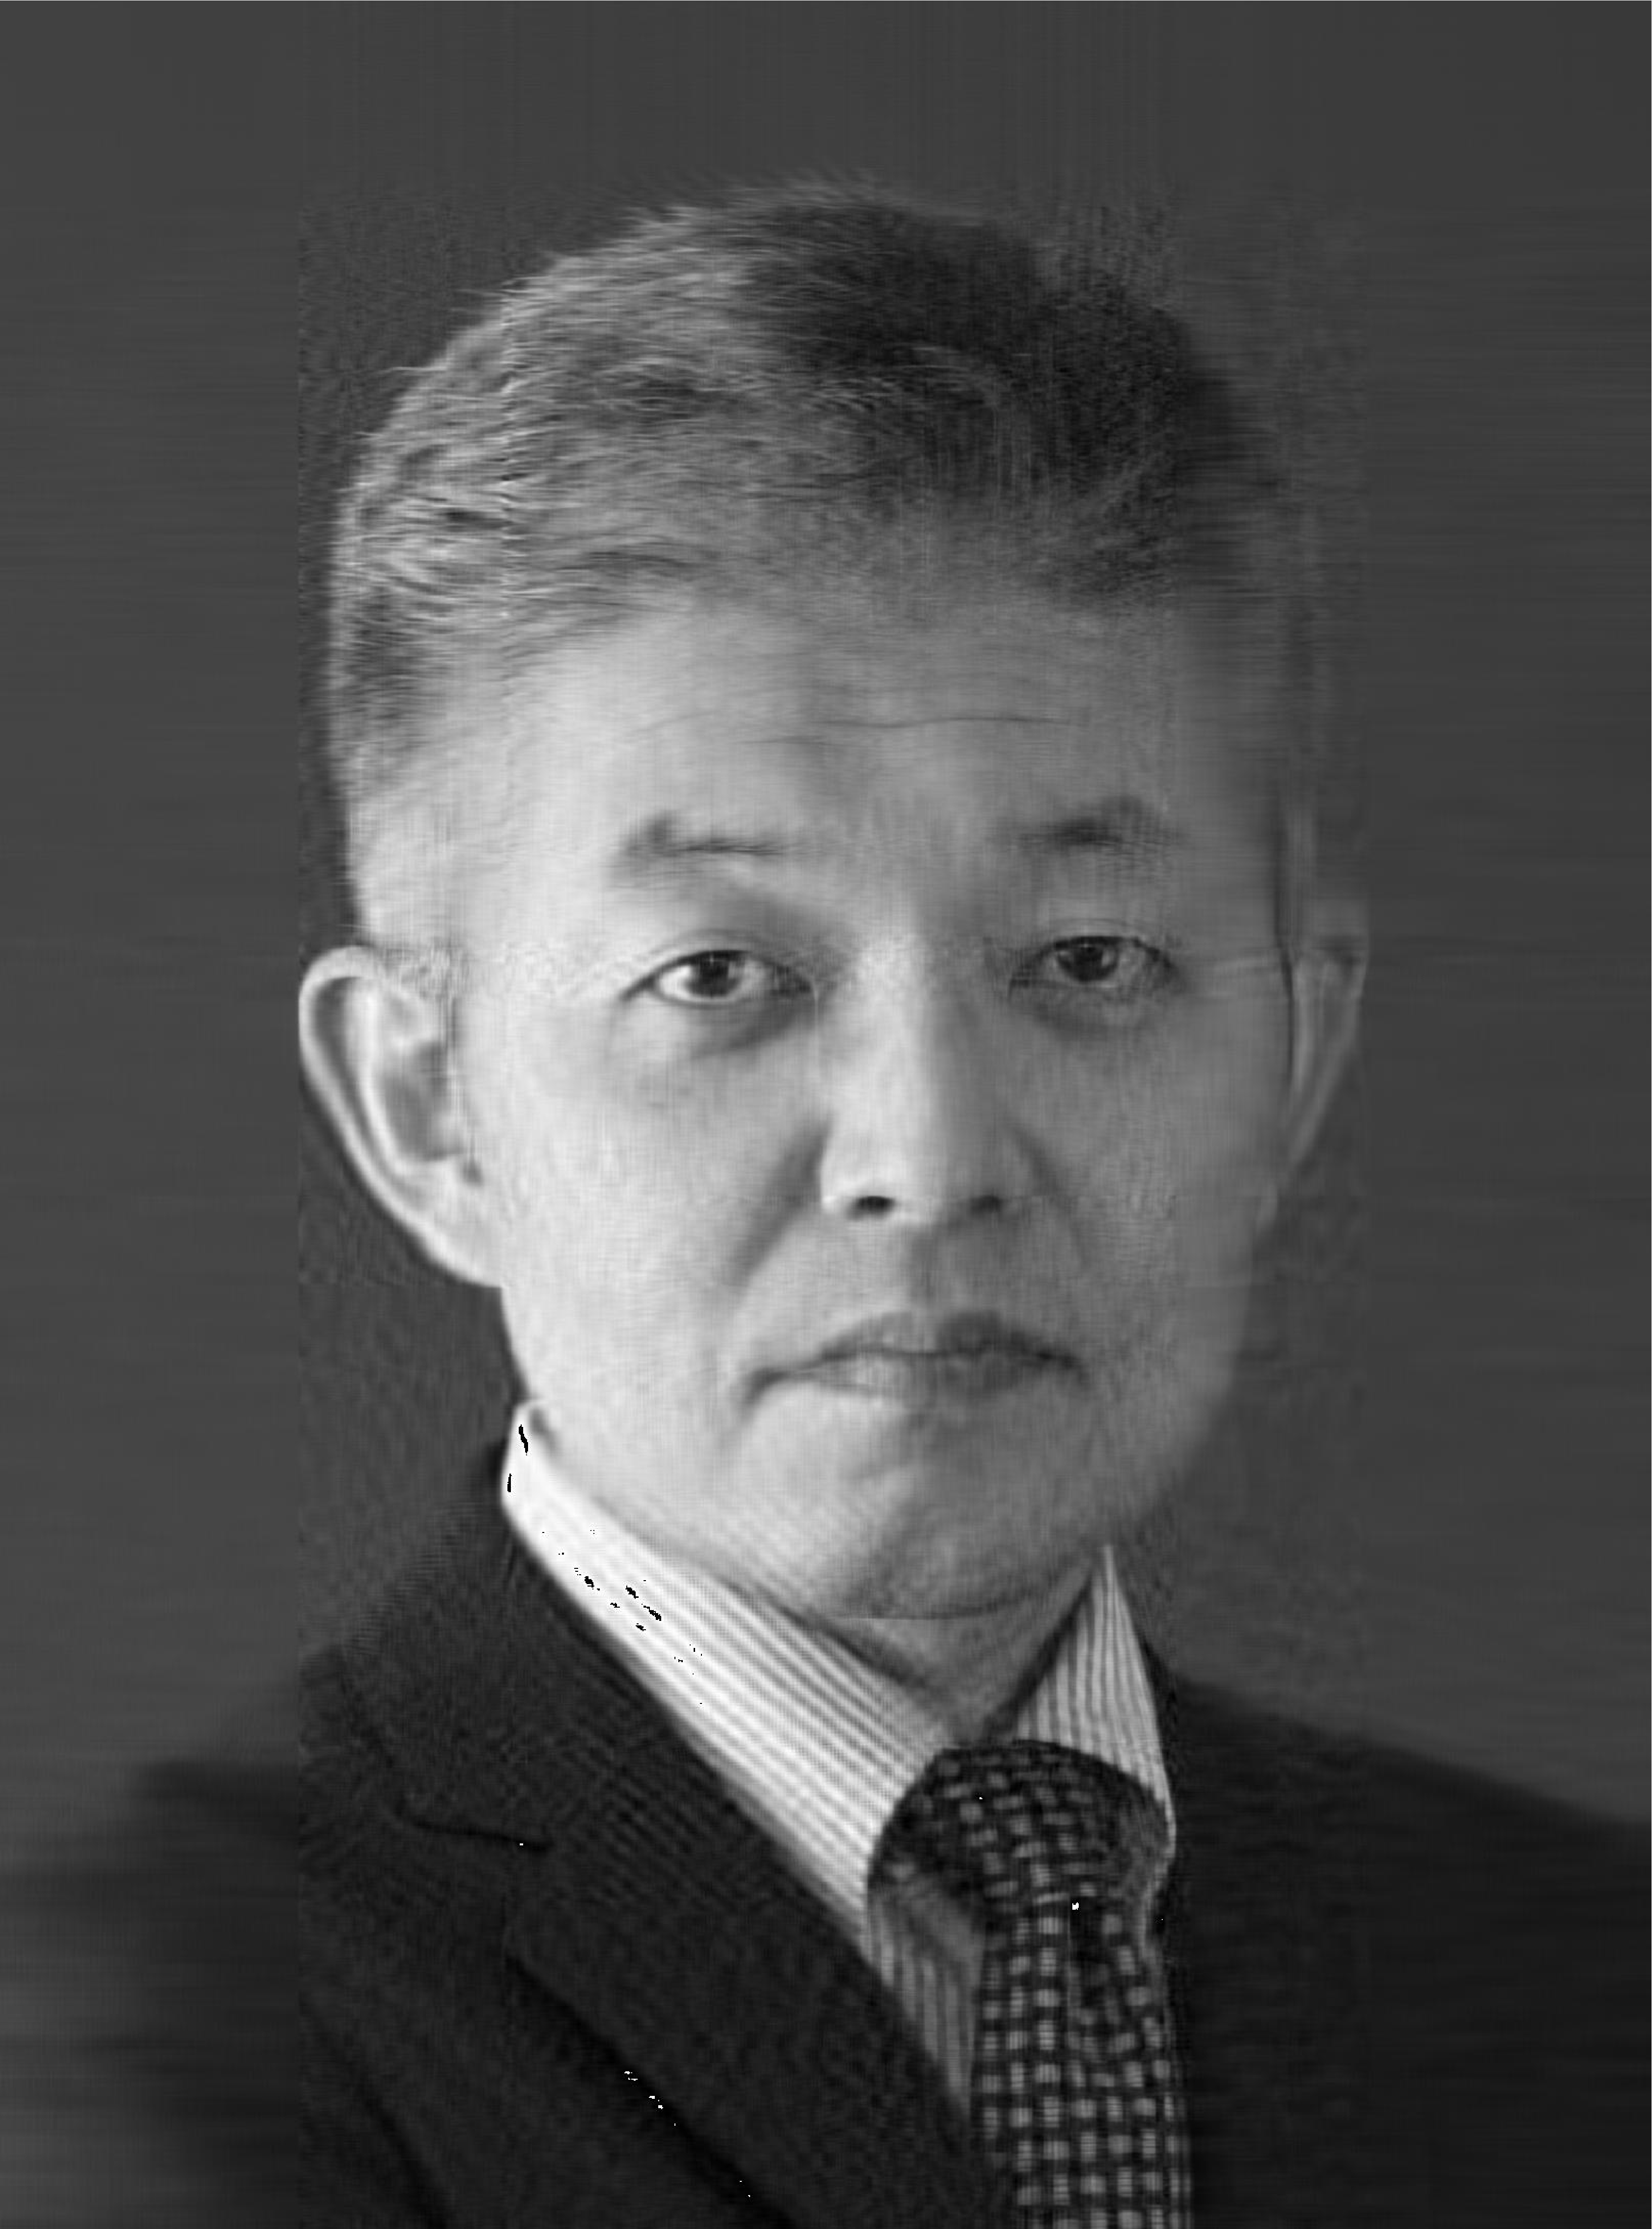
\includegraphics{image/gray_picture_r50.pdf}} \\
    \end{tabular}
  \end{itemize}
\end{frame}
